%% abtex2-modelo-relatorio-tecnico.tex, v-1.7.1 laurocesar
%% Copyright 2012-2013 by abnTeX2 group at http://abntex2.googlecode.com/ 
%%
%% This work may be distributed and/or modified under the
%% conditions of the LaTeX Project Public License, either version 1.3
%% of this license or (at your option) any later version.
%% The latest version of this license is in
%%   http://www.latex-project.org/lppl.txt
%% and version 1.3 or later is part of all distributions of LaTeX
%% version 2005/12/01 or later.
%%
%% This work has the LPPL maintenance status `maintained'.
%% 
%% The Current Maintainer of this work is the abnTeX2 team, led
%% by Lauro César Araujo. Further information are available on 
%% http://abntex2.googlecode.com/
%%
%% This work consists of the files abntex2-modelo-relatório-tecnico.tex,
%% abntex2-modelo-include-comandos and abntex2-modelo-references.bib
%%

% ------------------------------------------------------------------------
% ------------------------------------------------------------------------
% abnTeX2: Modelo de Relatório Técnico/Acadêmico em conformidade com 
% ABNT NBR 10719:2011 Informação e documentação - Relatório técnico e/ou
% científico - Apresentação
% ------------------------------------------------------------------------ 
% ------------------------------------------------------------------------

\documentclass[
	% -- opções da classe memoir --
	12pt,				% tamanho da fonte
% 	openright,			% capítulos começam em pág ímpar (insere página vazia caso preciso)
	oneside,			% para impressão em verso e anverso. Oposto a oneside
	a4paper,			% tamanho do papel. 
	% -- opções da classe abntex2 --
	%chapter=TITLE,		% títulos de capítulos convertidos em letras maiúsculas
	%section=TITLE,		% títulos de seções convertidos em letras maiúsculas
	%subsection=TITLE,	% títulos de subseções convertidos em letras maiúsculas
	%subsubsection=TITLE,% títulos de subsubseções convertidos em letras maiúsculas
	% -- opções do pacote babel --
	english,			% idioma adicional para hifenização
	french,				% idioma adicional para hifenização
	spanish,			% idioma adicional para hifenização
	brazil,				% o último idioma é o principal do documento
	]{abntex2}


% ---
% PACOTES
% ---
% Pacotes fundamentais 
% ---
\usepackage{cmap}				% Mapear caracteres especiais no PDF
\usepackage{lmodern}			% Usa a fonte Latin Modern
\usepackage[T1]{fontenc}		% Selecao de codigos de fonte.
\usepackage[utf8]{inputenc}		% Codificacao do documento (conversão automática dos acentos)
\usepackage{indentfirst}		% Indenta o primeiro parágrafo de cada seção.
\usepackage{color}				% Controle das cores
\usepackage{graphicx}			% Inclusão de gráficos
\usepackage{booktabs, multicol, multirow, hhline} % Esses includes fazem tabelas bem formatadas
\usepackage[table]{xcolor}
\usepackage{listings}
\usepackage{enumitem}
\usepackage{float}
\lstset{
    language=bash, %% Troque para PHP, C, Java, etc... bash é o padrão
    basicstyle=\ttfamily\small,
    numberstyle=\footnotesize,
    % numbers=left,
    % backgroundcolor=\color{gray!10},
    frame=single,
    tabsize=1,
    % rulecolor=\color{black!30},
    title=\lstname,
    escapeinside={\%*}{*)},
    breaklines=true,
    breakatwhitespace=true,
    framextopmargin=1pt,
    framexbottommargin=1pt,
    inputencoding=utf8,
    extendedchars=true,    
    literate={á}{{\'a}}1 {é}{{\'e}}1 {í}{{\'i}}1 {ó}{{\'o}}1 {ú}{{\'u}}1 
              {Á}{{\'A}}1 {É}{{\'E}}1 {Í}{{\'I}}1 {Ó}{{\'O}}1 {Ú}{{\'U}}1
              {à}{{\`a}}1 {è}{{\`e}}1 {ì}{{\`i}}1 {ò}{{\`o}}1 {ù}{{\`u}}1
              {À}{{\`A}}1 {È}{{\'E}}1 {Ì}{{\`I}}1 {Ò}{{\`O}}1 {Ù}{{\`U}}1
              {ä}{{\"a}}1 {ë}{{\"e}}1 {ï}{{\"i}}1 {ö}{{\"o}}1 {ü}{{\"u}}1
              {Ä}{{\"A}}1 {Ë}{{\"E}}1 {Ï}{{\"I}}1 {Ö}{{\"O}}1 {Ü}{{\"U}}1
              {â}{{\^a}}1 {ê}{{\^e}}1 {î}{{\^i}}1 {ô}{{\^o}}1 {û}{{\^u}}1
              {Â}{{\^A}}1 {Ê}{{\^E}}1 {Î}{{\^I}}1 {Ô}{{\^O}}1 {Û}{{\^U}}1
              {œ}{{\oe}}1 {Œ}{{\OE}}1 {æ}{{\ae}}1 {Æ}{{\AE}}1 {ß}{{\ss}}1
              {ű}{{\H{u}}}1 {Ű}{{\H{U}}}1 {ő}{{\H{o}}}1 {Ő}{{\H{O}}}1
              {ç}{{\c c}}1 {Ç}{{\c C}}1 {ø}{{\o}}1 {å}{{\r a}}1 {Å}{{\r A}}1
              {€}{{\euro}}1 {£}{{\pounds}}1 {«}{{\guillemotleft}}1
              {»}{{\guillemotright}}1 {ñ}{{\~n}}1 {Ñ}{{\~N}}1 {¿}{{?`}}1
              {_in}{{$\in$}}1 {_notin}{{$\notin$}}1 {_neq}{{$\neq$}}1
              {_textsubscript}{{\textsubscript{e=(u,v):u$\in$S}}}1
              {_textunderscore_}{{\textunderscore}}1
              {_textsubscript2}{{\textsubscript{e}}}1
}



% ---

% ---
% Pacotes adicionais, usados no anexo do modelo de folha de identificação
% ---
\usepackage{multicol}
\usepackage{multirow}

% ---
% Pacotes de citações
% ---
\usepackage[brazilian,hyperpageref]{backref}	 % Paginas com as citações na bibl
\usepackage[alf]{abntex2cite}	% Citações padrão ABNT

% --- 
% CONFIGURAÇÕES DE PACOTES
% ---
% Configurações do pacote backref
% Usado sem a opção hyperpageref de backref
\renewcommand{\backrefpagesname}{Citado na(s) página(s):~}
% Texto padrão antes do número das páginas
\renewcommand{\backref}{}
% Define os textos da citação
\renewcommand*{\backrefalt}[4]{
	\ifcase #1 %
		Nenhuma citação no texto.%
	\or
		Citado na página #2.%
	\else
		Citado #1 vezes nas páginas #2.%
	\fi}%
% ---

% ---
% Informações de dados para CAPA e FOLHA DE ROSTO
% ---
\titulo{Problema de Caminho-mais-Curto}
\autor{Alexandre Marangoni Costa \\ %author1
        André Luiz de Brandão Damasceno \\ %author2
        Antonio José Grandson Busson \\ %author3 
        Beatriz Marques Santiago%author4
    }

\local{Rio de Janeiro - RJ}
\data{2017}
\instituicao{%
  Pontíficia Universidade Católica do Rio de Janeiro
  \par
  Programa de Pós-Graduação em Informática}
\tipotrabalho{Relatório técnico}
% O preambulo deve conter o tipo do trabalho, o objetivo, 
% o nome da instituição e a área de concentração 
\preambulo{Relatório técnico apresentado como requisito
parcial para obtenção de aprovação na disciplina
Projeto e Análise de Algoritmos.}
% ---

% ---
% Configurações de aparência do PDF final

% alterando o aspecto da cor azul
\definecolor{blue}{RGB}{41,5,195}

% informações do PDF
\makeatletter
\hypersetup{
     	%pagebackref=true,
		pdftitle={\@title}, 
		pdfauthor={\@author},
    	pdfsubject={\imprimirpreambulo},
	    pdfcreator={LaTeX with abnTeX2},
		pdfkeywords={abnt}{latex}{abntex}{abntex2}{relatório técnico}, 
		colorlinks=true,       		% false: boxed links; true: colored links
    	linkcolor=blue,          	% color of internal links
    	citecolor=blue,        		% color of links to bibliography
    	filecolor=magenta,      		% color of file links
		urlcolor=blue,
		bookmarksdepth=4
}
\makeatother
% --- 

% --- 
% Espaçamentos entre linhas e parágrafos 
% --- 

% O tamanho do parágrafo é dado por:
\setlength{\parindent}{1.3cm}

% Controle do espaçamento entre um parágrafo e outro:
\setlength{\parskip}{0.2cm}  
% tente também \onelineskip

% ---
% compila o indice
% ---
\makeindex
% ---

% ----
% Início do documento
% ----
\begin{document}

% Retira espaço extra obsoleto entre as frases.
\frenchspacing 

% ----------------------------------------------------------
% ELEMENTOS PRÉ-TEXTUAIS
% ----------------------------------------------------------
% \pretextual

% ---
% Capa
% ---
\imprimircapa
% ---
\cleardoublepage
% ---
% Folha de rosto
% (o * indica que haverá a ficha bibliográfica)
% ---
\imprimirfolhaderosto*
% ---
\cleardoublepage
% ---
% Anverso da folha de rosto:
% ---

% ---
% inserir lista de ilustrações
% ---
% \pdfbookmark[0]{\listfigurename}{lof}
% \listoffigures*
% \cleardoublepage
% ---

% ---
% inserir lista de tabelas
% ---
% \pdfbookmark[0]{\listtablename}{lot}
% \listoftables*
% \cleardoublepage
% ---

% ---
% inserir lista de abreviaturas e siglas
% ---
% \begin{siglas}
%   \item[Fig.] Area of the $i^{th}$ component
%   \item[456] Isto é um número
%   \item[123] Isto é outro número
%   \item[lauro cesar] este é o meu nome
% \end{siglas}
% ---

% ---
% inserir lista de símbolos
% ---
% \begin{simbolos}
%   \item[$ \Gamma $] Letra grega Gama
%   \item[$ \Lambda $] Lambda
%   \item[$ \zeta $] Letra grega minúscula zeta
%   \item[$ \in $] Pertence
% \end{simbolos}
% ---

% ---
% inserir o sumario
% ---
\pdfbookmark[0]{\contentsname}{toc}
\tableofcontents*
\cleardoublepage
\include{abntex2-modelo-include-comandos}
% ---


% ----------------------------------------------------------
% ELEMENTOS TEXTUAIS
% ----------------------------------------------------------
\textual

% ----------------------------------------------------------
% Introdução
% ----------------------------------------------------------
\chapter*[Introdução]{Introdução}
\addcontentsline{toc}{chapter}{Introdução}
O problema do caminho mais curto consiste em determinar o menor custo de travessia entre dois ou mais pontos. Segundo \citeonline{tardos2005} o problema pode ser modelado utilizando teoria de grafos da seguinte forma: dado um grafo \textsf{G = (V,E)}, tal que \textsf{V} e \textsf{E} consistem respectivamente de uma coleção de vértices e arestas. Assumindo que para todo vértice \textsf{s} existe um caminho para qualquer outro vértice em \textsf{G}, e que para cada aresta \textsf{e} existe um valor \textsf{c\textsubscript{e} $\ge$ 0} indicando o tempo (ou distância, ou custo) associado à sua travessia. Um caminho \textsf{P} é definido pela soma dos valores de todas as arestas em \textsf{P}. O objetivo então é determinar o menor caminho de \textsf{s} para qualquer outro vértice no grafo.

O dijkstra é um dos algoritmos mais eficientes para encontrar o menor caminho em um grafo sem arestas com valores negativos. Sendo desenvolvido por Edsger W. Dijkstra em 1956 \cite{Misa:2010:IEW:1787234.1787249} e publicado em 1959 \cite{Dijkstra:1959:NTP:2722880.2722945}, o primeiro programa que utilizou o algoritmo tinha o objetivo de encontrar o caminho mais curto entre duas cidades na Holanda \cite{Misa:2010:IEW:1787234.1787249}. Na época foi utilizado um mapa reduzida da Holanda com apenas 64 cidades, onde cada cidade foi codificada utilizando apenas seis bits.
    
Conforme pode ser visto no pseudocódigo abaixo, a estrutura do algoritmo de Dijskstra se baseia em um conjunto \textsf{S} de vértices cujos os valores de caminhos mais curto \textsf{d(u)} desde a origem \textsf{s} já foram determinados. Inicialmente \textsf{S = \{s\}} e \textsf{d(s) = 0}. Para cada vértice \textsf{v $\in$ V-S} é determinado o caminho mais curto que pode ser feito passando pelas arestas exploradas de \textsf{S}. Assim, os passos são repetidos até que todos os vértices que possuem caminho a partir de \textsf{s} estejam em \textsf{S}.

\begin{lstlisting} %[caption=Pseudocódigo do algoritmo do Dijkstra, label=pseudoDijkstra]

Dijkstra (G,c)
Seja S um conjunto de vértices a serem explorados
    Para cada vértice u _in S, armazene uma distância d(u)    
Inicie S={S} e d(s)=0
Enquanto S _neq V
    Selecione um vértice v _notin S com ao menos uma aresta de S para
        d'(v) = min   _textsubscript    d(u) + c_textsubscript2 ser a menor possível        
    Adicione v em S e defina d(v) = d'(v)    
\end{lstlisting}

O dijkstra tem a característica de ser um algoritmo guloso, ou seja, toma a decisão do caminho mais curto que parece ser a melhor no momento de cada iteração. A corretude de que para todo vértice \textsf{u $\in$ S}, o caminho \textsf{P\textsubscript{u}} é o mais curto, pode ser feita por indução do tamanho de \textsf{S}. Supondo que a afirmação seja mantida quando \textsf{|S| = k} para qualquer valor de \textsf{k $\ge$ 1}. Aumentando \textsf{S} para o tamanho de \textsf{k + 1} através da adição do vértice \textsf{v}, a aresta \textsf{(u,v)} passa a ser a aresta final do caminho \textsf{P\textsubscript{v}} do vértice \textsf{s} ao \textsf{v}. Baseado na hipótese de indução, \textsf{P\textsubscript{u}} é o caminho mais curto para cada vértice \textsf{u $\in$ S}. Agora considerando um outro caminho \textsf{P} de \textsf{s} até \textsf{v}, deseja-se mostrar que ele possui pelo menos o mesmo tamanho de \textsf{P\textsubscript{v}}. Para alcançar \textsf{v}, esse caminho \textsf{P} deve sair pelo conjunto \textsf{S} através de \textsf{y}, o primeiro vértice em \textsf{P} que não está em \textsf{S}, e \textsf{x $\in$ S} o vértice anterior ao \textsf{y}. Essa situação pode ser vista na Figura \ref{fig:graph}.

\begin{figure}[!ht]
 \centering
 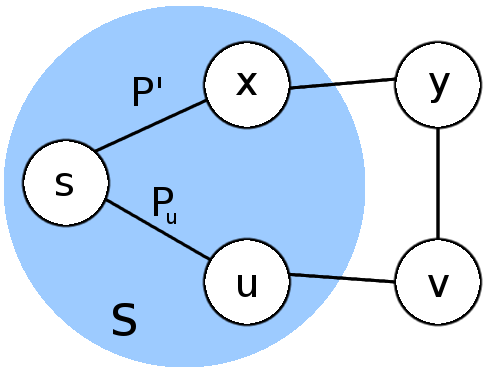
\includegraphics[width=2.4in]{graph.png}
 \caption{Caminho mais curto \textsf{P\textsubscript{v}} e um caminho \textsf{P} alternativo do vértice \textsf{s} ao \textsf{v} através do vértice \textsf{y}.}
 \label{fig:graph}
\end{figure}

Entretanto, \textsf{P} não pode ser menor do que \textsf{P\textsubscript{v}} porque ele já é pelo menos do tamanho de \textsf{P\textsubscript{v}}. Na iteração \textsf{k + 1}, o algoritmo de Dijkstra deve ter considerado adicionar o vértice \textsf{y} para o conjunto \textsf{S} via aresta \textsf{(x,y)}, e rejeitou essa opção em favor da adição de \textsf{v}. Isso significa que não existe caminho de \textsf{s} a \textsf{y} por meio de \textsf{x} que seja mais curto do que \textsf{P\textsubscript{v}}. A prova desse argumento pode ser feita utilizando inequações. Sabendo que \textsf{x $\in$ S}, \textsf{P'} é um subgrafo de \textsf{P} e o caminho de \textsf{s} à \textsf{x} está contido em \textsf{P'}, sabe-se por hipótese de indução que \textsf{P\textsubscript{x}} é o caminho mais curto de \textsf{s} à \textsf{x} (de tamanho \textsf{d(x)}), logo \textsf{c(P') $\ge$ c(P\textsubscript{x}) = d(x)}. Assim o subgrafo de \textsf{P} até \textsf{y} tem tamanho \textsf{c(P') + c(x,y) $\ge$ d(x) + c(x,y) $\ge$ d'(y)}, e o caminho completo de P é pelo menos do mesmo tamanho desse subgrafo. Desde que o dijkstra selecione \textsf{v} nessa iteração, sabe-se que \textsf{d'(y) $\ge$ d'(v) = c(P\textsubscript{v})}. Combinando essas inequações pode-se mostrar que \textsf{c(P) $\ge$ c(P') + c(x,y) $\ge$ c(P\textsubscript{v})}.

% Considerando que os vértices e suas respectivas distâncias são uma fila de prioridade em que sempre o próximo vértice com menor distancia terá maior prioridade, o tempo de execução da inserção de vértices nesta lista de prioridade, mudança de chaves e deleção do mínimo define a complexidade do dijkstra. Isso pode ser observado na seguinte tabela:

%(André) acho melhor falar sobre a complexidade de cada operação (inserir, remover mínimo, etc.) da estruturas (vetor, arvore, etc.) na seus respectivos capítulos. Acredito que isso seja melhor porque a complexidade de algumas operações depende muito da forma que ela foram implementadas.

% \begin{table}[ht!]
%   \centering    
%   \begin{tabular}{r|c|c|c}
%     \toprule
%     Estrutura & inserção & mudança de chave & deleção minimo\\
%     \midrule
%     Vetor & O(1) & O(1) & O(n)\\
%     \hline
%     AVL & O(logn) & O(1) & O(logn)\\
%     \hline
%     Fibonacci heap & O(1)(amortizado) & O(1)(amortizado) & O(logn)\\
%     \hline
%     Buckets & O(1) & O(1) & O(n)\\
%     \hline
%     Arvore $\alpha$ & ? & ? & ?\\
%   \end{tabular} 
%   \caption{Complexidade por estrutura de dados}  
%   \label{tab:table1}
% \end{table}

A complexidade em tempo de execução do Dijkstra é altamente relacionada com a estrutura de dados usada nesta etapa:

\begin{lstlisting}
Selecione um vértice v _notin S com ao menos uma aresta de S para
    d'(v) = min   _textsubscript    d(u) + c_textsubscript2 ser a menor possível
\end{lstlisting}

A fim de analisar diferentes cenários, este relatório apresenta detalhes sobre as complexidades usando 5 tipos de estruturas de dados diferentes: vetor, árvore balanceada de busca, heap de Fibonacci, buckets e árvore $\alpha$.
Cada estrutura foi dividida em um capítulo, e em cada capítulo será apresentado um código diferente do original, modificando principalmente o trecho acima para ilustrar a estrutura de dados analisada.

%(Alexandre) acho desnecessário isso.
%O Capítulo 1 descreve o algoritmo utilizando um vetor. O Capítulo 2 descreve a utilização de uma Árvore Balanceada AVL. O Capítulo 3 analisa o algoritmo utilizando uma \textit{Heap de Fibonacci}. O Capítulo 4 apresenta o Dijsktra utilizando \textit{Buckets}. O Capítulo 5 mostra o algoritmo utilizando uma Árvore $\alpha$. O Capítulo 6 apresenta os resultados obtidos nos testes executados com as diferentes estruturas de dados descritas. Por último, são apresentadas as considerações finais.


\chapter{Estruturas de dados}
% \section{Aliquam vestibulum fringilla lorem}

A Listagem \ref{struct.vertice} ilustra a estrutura utilizada para armazenar os dados dos vértice. O atributo \emph{index} informa o índice do vértice; O atributo \emph{distance} informa a distancia mínima até o vértice de partida, durante a inicialização do algoritmo, este atributo recebe o valor da macro INT\_MAX da biblioteca \textsf{limits.h}, o qual simboliza o valor $\infty$; O atributo \emph{adjs} faz referencia aos vértices adjacentes; E por último, o atributo \emph{weights} faz referencia aos pesos das arestas.

\begin{lstlisting}[caption=Estrutura de um vértice, label=struct.vertice]
 struct vertice{
   guint32 index;
   guint32 distance;
   struct vertice** adjs;
   guint32* weights;
 };
\end{lstlisting}


\section{Vetor}
Conforme visto na introdução, o algoritmo do Dijkstra é um algoritmo guloso, que usa uma estrutura de dados para armazenar as menores distâncias conhecidas a cada iteração. Portanto, inserir, remover e atualizar os elementos dessa estrutura são as operações que mais influenciam a complexidade final. Ilustraremos isso com o seguinte pseudo-código \cite{dasgupta2006}, onde \textsf{G} representa o grafo, \textsf{l} guarda o custo de cada aresta, e \textsf{s} é o nó inicial de onde dijkstra partirá.

\begin{lstlisting}[mathescape=true, label=dijkstra.pseudo.vetor]
Dijkstra (G, l, s)
para todo u em G.vertices
    dist[u] = $\infty$
    
dist[s] = 0
vetor = cria_vetor(dist)       

enquanto vetor != $\emptyset$
    u = remove_min(vetor)
    para todo (u, v) em G.arestas
        se dist[v] > dist[u] + l(u, v)
            dist[v] = dist[u] + l (u, v)
            atualiza_chave(vetor, v, dist[v])
\end{lstlisting}

Inicialmente, o algoritmo percorre os vértices para inicializar o vetor de distâncias (resultado final) e cria a estrutura de dados que armazena as distâncias conhecidas a cada passo guloso. Neste capítulo, essa estrutura também é um vetor, então para acessar um elemento através de um índice, gasta-se \textsf{O(1)}. Para inicializar n vértices gasta-se n operações. Portanto a complexidade destes primeiros passos é \textsf{n} x \textsf{O(1)} = \textsf{O(n)}.

Em seguida, o algoritmo deve remover o menor elemento do vetor, o vértice \textsf{u}. O vetor não está ordenado, então a busca de \textsf{u} ocorre em \textsf{O(n)} operações. Além disso, esse passo remove cada vértice do vetor um a um. Como temos n vértices, temos \textsf{O(n)} operações que custam \textsf{O(n)}, resultando em \textsf{O($n^2$)} operações.

Por fim, caso encontremos um vértice \textsf{v} com aresta para \textsf{u} (do passo anterior) através de um caminho melhor do que conhecíamos previamente, atualizamos a distância que conhecemos até o vértice \textsf{v}. Atualizar o elemento de um vetor custa O(1). Como isso é feito uma vez para cada aresta do grafo, em um grafo de m arestas, temos \textsf{O(m)} operações. Além disso, assumindo que um grafo possa conter no máximo O($n^2$) arestas, a complexidade do pior caso é \textsf{O($n^2$)}.

%Esta implementação usa um vetor não ordenado cujo índice identifica o vértice e o valor representa a distância entre o vértice origem \textsf{s} e o vértice em questão. Como pode ser visto na Listagem \ref{dijkstra.vetor}, a cada iteração, o algortimo Dijkstra deve obter o vértice com a menor distancia (Passo 1.1). Para isso, é necessario percorrer todo o vetor, o que resulta em \textsf{n} x \textsf{O(n)} operações, onde \textsf{n} é igual ao número de vértices. A atualização das distancias (Passo 1.3) é feita para diretamente para vértice adjacente, o que resulta em \textsf{m} x \textsf{O(1)} operações, onde \textsf{m} é igual ao número de arestas.

\textbf{Conclui-se que a complexidade total do Dijkstra com vetor é O($n^2$).}

Abaixo temos esse trecho implementado em C. No código abaixo, \emph{vertices} é o \emph{G.vertices} do pseudo código, e \emph{v->distance} (veja \ref{struct.vertice} acima) substitui o vetor \emph{dist} do pseudo código. Ambos já estão inicializados, e o resto do código pode ser facilmente mapeado ao pseudo-código linha a linha:

\begin{lstlisting}[caption=Corpo do algortimo Dijkstra com uso do vetor, label=dijkstra.vetor]
 for(guint32 count = 0; count < numVertices; count++){
     vertice* v = get_min_distance(vertices); /* 1.1 */
      
     for(guint32 i=0;i< v->adjCount;i++){  /* 1.3 */
         vertice * w = vertices[v->adjs[i]->index];
         if(v->distance + v->weights[i] < w->distance)
            w->distance = v->distance + v->weights[i]; 
     }
 }
\end{lstlisting}


\section{Árvore Balanceada de Busca}
Em uma árvore balanceada de busca, a altura da árvore é constantemente balanceada, possuindo sempre um valor proporcional a \textsf{O($log(n)$)}. Para buscar elementos, bem como a encontrar a posição correta de um elemento nessa estrutura, percorre-se as alturas, uma a uma. Portanto, temos que a complexidade de se inserir/remover/atualizar um elemento é \textsf{O($log(n)$)}.

Assim sendo, usando o mesmo pseudo código acima, mas trocando vetor por essa nova estrutura, podemos ver que inicialmente o algoritmo inicializa os n vértices em \textsf{O($n.log(n)$)} operações.

Em seguida, o algoritmo remove cada vértice, também em \textsf{O($n.log(n)$)} operações.

Por último, para cada nova aresta conhecida (m arestas), o algoritmo guloso atualiza o vértice destino na árvore balanceada, de acordo com a nova distância revelada por essa nova aresta, em \textsf{O($log(n)$)}. Temos aqui \textsf{O($m.log(n)$)} operações.

\textbf{Portanto, a complexidade do Dijkstra usando uma árvore balanceada de busca é O((n+m).log(n)).}

A implementação em C apresentada neste trabalho usa uma árvore balanceada binária, a variável \emph{tree}, que corresponde à variável \emph{vetor} do pseudo código. Ao invés de inicializar essa árvore com todos os vértices, eles são inseridos apenas quando o algoritmo guloso chega até eles. Para buscar, remover e inserir elementos na árvore, são usadas as funções g\_tree\_search, g\_tree\_remove e g\_tree\_insert respectivamente, e o restante do algoritmo pode ser facilmente compreendido.

\begin{lstlisting}[caption=Corpo do algoritmo Dijkstra com uso da árvore balanceada de busca, label=dijkstra.arvore]
 while(g_tree_height(tree)>0){  
    vertice* v = g_tree_search(tree,&query); /* 1.1 */
    g_tree_remove(tree,v);  

    for(guint32 i=0;i<v->adjCount;i++){ /* 1.3 */
        vertice * w = v->adjs[i];
        if(v->distance + v->weights[i] < w->distance){
           w->distance = v->distance + v->weights[i];
           g_tree_textunderscore_insert(tree,w);
        } 
    }
 }    
\end{lstlisting}

\section{Heap de Fibonacci}

Uma análise análoga a anterior pode ser feita para o Heap de Fibonacci. Remover o menor elemento do heap (função heap\_extract\_min) custa O(log(n)) para um grafo de n vértices. Já inserir no heap de fibonacci (heap\textunderscore insert) custa O(1) (amortizado) \cite{dasgupta2006}.

A implementação em C do algoritmo insere os vértices no heap a medida em que eles vão sendo descobertos. Além disso, todos os vértices já são inicializados com distância $\infty$. Portanto, o trecho do pseudo código que interessa analizar é o seguinte:

\begin{lstlisting}[caption=parte do Pseudo-código do algoritmo de Dijkstra, mathescape=true, label=dijkstra.pseudo.heap]
enquanto heap != $\emptyset$
    u = remove_min(heap)
    para todo (u, v) em G.arestas
        se dist[v] > dist[u] + l(u, v)
            dist[v] = dist[u] + l (u, v)
            atualiza_chave(heap, v, dist[v])
\end{lstlisting}

Inicialmente os n vértices são removidos do heap um a um, quando sua distância mínima é encontrada. Como remover do heap de Fibonacci custa $O(log(n))$, este passo custa $O(n.log(n))$ no total.

Além disso, para cada aresta de um grafo com m arestas, são feitas algumas operações em $O(1)$ e, ocasionalmente, atualizações de chave, em $O(1)$ amortizado. O que nos dá uma complexidade amortizada de $O(m)$

\textbf{Portanto, a complexidade amortizada total é O(n.log(n) + m).}

Na implementação em C apresentada, ao invés de atualizarmos uma chave, é feita a inserção do nó corrente, que também é $O(1)$ amortizado. Portanto a complexidade final é a mesma.

\begin{lstlisting}[caption=Corpo do algortimo Dijkstra com uso da heap de fibonacci, label=dijkstra.heap]
 while (!is_empty(heap)){
    vertice * v = heap_extract_min(heap); /* 1.1 */

    for(guint32 i=0;i< v->adjCount;i++){ /* 1.3 */
       vertice * w = v->adjs[i];
       if(v->distance + v->weights[i] < w->distance){
          w->distance = v->distance + v->weights[i];
          heap_textunderscore_insert(heap,w);
       } 
    }
 }   
\end{lstlisting}



\section{Buckets}

A implementação do algoritmo de Dijkstra usando Buckets é identica a usando o Heap de Fibonacci, e a sua complexidade pode ser analisada de forma análoga, conforme veremos adiante.

Veja o código abaixo:

\begin{lstlisting}[caption=Corpo do algortimo Dijkstra com uso de buckets, label=dijkstra.buckets]
 while(!bucket_is_empty(buc)){
    vertice* v = bucket_remove_min(buc); /* 1.1 */
   
    for(guint32 i=0;i< v->adjCount;i++){ /* 1.3 */
      vertice * w = v->adjs[i];
      if(v->distance + v->weights[i] < w->distance){
         w->distance = v->distance + v->weights[i];   
         bucket_add(buc,w);
      } 
    }
 }   
\end{lstlisting}

Inicialmente, o algoritmo remove o vértice com menor distância dos buckets, uma vez para cada vértice. Remover o mínimo elemento dos buckets custa O(C) amortizado, onde C é o valor máximo do custo de uma aresta. Assim sendo, a complexidade amortizada deste passo é O(nC).

Em seguida, para cada aresta o algoritmo faz algumas operações em O(1) e, eventualmente, insere um elemento nos buckets. Inserir nos buckets custa O(1). Portanto este passo custa O(m).

\textbf{No total, podemos ver que o algoritmo de Dijkstra implementado com buckets tem complexidade O(nC + m).}

\section{Árvore $\alpha$}

BB[$\alpha$] tree, ou simplesmente Árvore $\alpha$, é um tipo de árvore binária de busca com auto-balancemanto, introduzida pela primeira vez em \cite{nievergelt1973binary}. Na árvore $\alpha$ o tamanho de um nó interno é a soma do tamanho de seus dois filhos mais um (size[n] = size[n.left] + size[n.right] + 1). Um nó da árvore $\alpha$ é dito balanceado se: size[n.left] $\le$ $\alpha$.size[n] e size[n.right] $\le$ $\alpha$.size[n].

\begin{enumerate}
  \item Caso seja necessário realizar o balanceamento da árvore $\alpha$, pega-se o \textsf{v} mais alto que não é $\alpha$-balanceado, então a sub-árvore de \textsf{v} é trocada por uma sub-árvore $\alpha$-balanceada que contém os mesmos elementos. Para realizar o balanceamento checa-se cada elemento da sub-árvore, obtendo assim O(size[x]) operações. 
  \item Para a operação de busca, no pior caso (quando o nó é uma folha) é preciso percorrer apenas um nó por nível, até chegar na folha. Quando $\alpha$ é próximo de 1/2 a árvore $\alpha$ tem um comportamento semelhante a uma árvore binária de busca, que no pior caso tem uma complexidade O(log(n)). Já quando $\alpha$ é próximo a 1 a árvore $\alpha$ tem um comportamento semelhante a uma lista, que no pior caso tem complexidade O(n).  
  \item A partir daqui considere alpha estritamente maior que 1/2.
  \item Dependendo como os nós de uma árvore binária de busca estão distribuídos, o potencial pode ser maior que zero, por exemplo quando uma árvore degenera para uma lista crescente, tem-se que para todo nó \textsf{n}, size[n.left] = 0 e size[n.right] = 1. Já para uma árvore 1/2-balanceada, tem-se que o tamanhos dos filhos esquerdo e direito são os mesmos (size[n.left] = size[n.right]), pois ambos devem ter um tamanho maior que a metade de size[n]. Caso contrário, a condição de balanceamento $\alpha$ não esta satisfeita. Logo, o potencial é igual a ZERO.
  \item Quando a árvore degenera para uma lista (com $\alpha$ próximo a 1), o balanceamento pode ser feito com apenas 1 troca de seus filhos, resultando em O(1) operações para balancear uma sub-árvore.
  \item Para a operação de inserção na árvore $\alpha$ é necessário percorrer um nó por nível até que a folha seja alcançada (vide item ii), o que resulta em O(log(n)) operações. Caso seja necessário fazer o balanceamento da árvore (vide item i) é gasto O(size[v]) operações, onde \textsf{v} é o nó raiz da sub-arvore balanceada. O que resulta em uma complexidade que varia de O(log(n) + size[v])) até O(n), dependendo do valor de $\alpha$ Como a árvore $\alpha$ dificilmente degenera para uma lista, obtém-se uma complexidade amortizada de O(log(n)). Para a operação de deleção é feito um processo semelhante, com a diferença que quando o nó a ser deletado é encontrado, deve-se exclui-lo, colocando em seu lugar um de seus filhos de forma que o balanceamento seja mantido. Como na operação de inserção, a deleção também tem complexidade amortizada de O(log(n)).  
\end{enumerate}

\textbf{Portanto, a complexidade do Dijkstra usando uma árvore $\alpha$ pode variar de O((n+m).log(n)) até O($n^2$), dependendo do valor de $\alpha$.}

A implementação em C apresentada neste trabalho usa uma árvore $\alpha$, que ao invés de
inicializar essa árvore com todos os vértices, eles são inseridos apenas quando o algoritmo
guloso chega até eles. Para remover o menor e inserir elementos na árvore, são usadas as
funções alpha\_tree\_smallest e alpha\_tree\_insert respectivamente, e o restante do
algoritmo pode ser facilmente compreendido.
\\
\\
\\
\begin{lstlisting}[caption=Corpo do algortimo Dijkstra com uso da árvore $\alpha$, label=dijkstra.alpha]
 while(alpha_tree_height(tree)>0){
    vertice* v = alpha_tree_smallest(tree); /* 1.1 */
      
    for(guint32 i=0;i< v->adjCount;i++){ /* 1.3 */
      vertice * w = v->adjs[i];
      if(v->distance + v->weights[i] < w->distance){
         w->distance = v->distance + v->weights[i];   
         alpha_textunderscore_tree_textunderscore_insert(tree,w);
      } 
    }
 } 
\end{lstlisting}

\chapter{Resultados}
Para realizar o experimento de execução do dijkstra foram utilizados máquinas de mesma configuração com processador Intel Core i7-6700 3,4 GHz x 8, memória de 15,6 GB e sistema operacional ubuntu 16.04 LTS na versão 64 bits. Os algoritmos foram implementados utilizando a linguagem C e compilados através do gcc 5.4.0.

Os dados dos grafos utilizados estavam em arquivos no formato STP dividos em pastas chamadas ALUE, ALUT e DMXA. Cada arquivo apresentava a quantidade de vértices e arestas. Cada aresta era especificada pelo valor do vértice de origem, destino e custo de travessia. O vértice \textsf{1} de cada um dos arquivos foi definido como o vértice de origem do dijkstra. Para a análise foi assumido que n = V (número de vértices)  e m = E (número de arestas). 

Os resultados das execuções do dijkstra em cada uma das estrutura de dados (Vetor, Árvore Balanceada de Busca, Heap de Fibonacci, Buckets e Árvore $\alpha$), podem ser observados nas tabelas e gráficos abaixo. Em geral todas as tabelas estão com seus resultados ordenados pelo número de vértices dos grafos. Em todas as tabelas, tem suas colunas organizadas pelo nome do arquivo, numero de vértices e arestas, quantidade de vértices processados, tempo de execução e complexidade teórica. A tabela de Árvore $\alpha$, além de apresentar as mesmas colunas das outras estruturas de dados, com exceção da coluna de complexidade teórica, mostra os valores do tempo de execução com diferentes valores para $\alpha$. \\

\begin{table}[H]
  \centering    
  \begin{tabular}{|c|r|r|r|r|r|}
    \toprule
    \multicolumn{5}{|c|}{\cellcolor{gray!25}\textbf{Vetor}} & \cellcolor{gray!25}\textbf{Complexidade Teórica}\\
    \midrule
    \multicolumn{1}{|c|}{\cellcolor{gray!10}Arquivo} & \multicolumn{1}{|c|}{\cellcolor{gray!10}Vértices} & \multicolumn{1}{|c|}{\cellcolor{gray!10}Arestas} & \multicolumn{1}{|c|}{\cellcolor{gray!10}V. Processados} & \multicolumn{1}{|c|}{\cellcolor{gray!10}Tempo} & \multicolumn{1}{|c|}{\cellcolor{gray!10}|V|\textsuperscript{2}}\\
    % \midrule
    \hline
    alue7229 & 940 & 1474 & 940 & 0,002559 & 883600\\
    \hline
    alue2105 & 1220 & 1858 & 1858 & 0,005142 & 1488400\\
    \hline
    alue2087 & 1244 & 1971 & 1971 & 0,005306 & 1547536\\
    \hline
    alue6951 & 2818 & 4419 & 4419 & 0,045333 & 7941124\\
    \hline
    alue6179 & 3372 & 5213 & 5213 & 0,068000 & 11370384\\
    \hline
    alue5067 & 3524 & 5560 & 5560 & 0,076727 & 12418576\\
    \hline
    alue3146 & 3626 & 5869 & 5869 & 0,078092 & 13147876\\
    \hline
    alue6457 & 3932 & 6137 & 6137 & 0,112444 & 15460624\\
    \hline
    alue6735 & 4119 & 6696 & 6696 & 0,114364 & 16966161\\
    \hline
    alue5623 & 4472 & 6938 & 6938 & 0,138595 & 19998784\\
    \hline
    alue5345 & 5179 & 8165 & 8165 & 0,206080 & 26822041\\
    \hline
    alue7066 & 6405 & 10454 & 10454 & 0,348000 & 41024025\\
    \hline
    alue5901 & 11543 & 18429 & 18429 & 1,233600 & 133240849\\
    \hline
    alue7065 & 34046 & 54841 & 54841 & 2,874000 & 1159130116\\
    \hline
    alue7080 & 34479 & 55494 & 55494 & 2,996000 & 1188801441\\
    \hline
  \end{tabular}
  \caption{Tabela de resultados do ALUE utilizando Vetor.}  
  \label{tab:AlueVetor}
\end{table}

\begin{table}[H]
  \centering    
  \begin{tabular}{|c|r|r|r|r|r|}
    \toprule
    \multicolumn{5}{|c|}{\cellcolor{gray!25}\textbf{Árvore Balanceada de Busca}} & \cellcolor{gray!25}\textbf{Complexidade Teórica}\\
    \midrule
    \multicolumn{1}{|c|}{\cellcolor{gray!10}Arquivo} & \multicolumn{1}{|c|}{\cellcolor{gray!10}Vértices} & \multicolumn{1}{|c|}{\cellcolor{gray!10}Arestas} & \multicolumn{1}{|c|}{\cellcolor{gray!10}V. Processados} & \multicolumn{1}{|c|}{\cellcolor{gray!10}Tempo} & \multicolumn{1}{|c|}{\cellcolor{gray!10}(|V|+|E|)log|V|}\\
    % \midrule
    \hline
    alue7229	&	940	&	1474	&	809	&	0,001171	&	23841,91	\\
    \hline
    alue2105	&	1220	&	1858	&	896	&	0,001403	&	31557,70	\\
    \hline
    alue2087	&	1244	&	1971	&	933	&	0,001410	&	33052,68	\\
    \hline
    alue6951	&	2818	&	4419	&	2035	&	0,003392	&	82939,32	\\
    \hline
    alue6179	&	3372	&	5213	&	2748	&	0,004204	&	100610,95	\\
    \hline
    alue5067	&	3524	&	5560	&	2975	&	0,005062	&	107036,76	\\
    \hline
    alue3146	&	3626	&	5869	&	2852	&	0,004501	&	112270,43	\\
    \hline
    alue6457	&	3932	&	6137	&	3578	&	0,005741	&	120234,41	\\
    \hline
    alue6735	&	4119	&	6696	&	2970	&	0,004689	&	129867,37	\\
    \hline
    alue5623	&	4472	&	6938	&	2750	&	0,004470	&	138365,70	\\
    \hline
    alue5345	&	5179	&	8165	&	4215	&	0,007176	&	164644,38	\\
    \hline
    alue7066	&	6405	&	10454	&	4767	&	0,008124	&	213181,77	\\
    \hline
    alue5901	&	11543	&	18429	&	8579	&	0,014905	&	404464,07	\\
    \hline
    alue7065	&	34046	&	54841	&	31374	&	0,075032	&	1338211,36	\\
    \hline
    alue7080	&	34479	&	55494	&	34479	&	0,082340	&	1356201,75	\\
    \hline
  \end{tabular}
  \caption{Tabela de resultados do ALUE utilizando Árvore Balanceada de Busca.}  
  \label{tab:AlueArvore}
\end{table}

\begin{table}[H]
  \centering    
  \begin{tabular}{|c|r|r|r|r|r|}
    \toprule
    \multicolumn{5}{|c|}{\cellcolor{gray!25}\textbf{Heap de Fibonacci}} & \cellcolor{gray!25}\textbf{Complexidade Teórica}\\
    \midrule
    \multicolumn{1}{|c|}{\cellcolor{gray!10}Arquivo} & \multicolumn{1}{|c|}{\cellcolor{gray!10}Vértices} & \multicolumn{1}{|c|}{\cellcolor{gray!10}Arestas} & \multicolumn{1}{|c|}{\cellcolor{gray!10}V. Processados} & \multicolumn{1}{|c|}{\cellcolor{gray!10}Tempo} & \multicolumn{1}{|c|}{\cellcolor{gray!10}|V|log|V| + E}\\
    % \midrule
    \hline
    alue7229	&	940	&	1474	&	809	&	0,000558	&	10757,93	\\
    \hline
    alue2105	&	1220	&	1858	&	896	&	0,000610	&	14366,25	\\
    \hline
    alue2087	&	1244	&	1971	&	933	&	0,000641	&	14760,28	\\
    \hline
    alue6951	&	2818	&	4419	&	2035	&	0,001475	&	36714,56	\\
    \hline
    alue6179	&	3372	&	5213	&	2748	&	0,002002	&	44730,78	\\
    \hline
    alue5067	&	3524	&	5560	&	2975	&	0,002233	&	47083,29	\\
    \hline
    alue3146	&	3626	&	5869	&	2852	&	0,002129	&	48743,42	\\
    \hline
    alue6457	&	3932	&	6137	&	3578	&	0,002734	&	53089,20	\\
    \hline
    alue6735	&	4119	&	6696	&	2970	&	0,002201	&	56157,27	\\
    \hline
    alue5623	&	4472	&	6938	&	2750	&	0,002046	&	61168,62	\\
    \hline
    alue5345	&	5179	&	8165	&	4215	&	0,003262	&	72065,87	\\
    \hline
    alue7066	&	6405	&	10454	&	4767	&	0,003693	&	91445,12	\\
    \hline
    alue5901	&	11543	&	18429	&	8579	&	0,006775	&	174198,68	\\
    \hline
    alue7065	&	34046	&	54841	&	31374	&	0,032623	&	567410,26	\\
    \hline
    alue7080	&	34479	&	55494	&	34479	&	0,035800	&	575210,80	\\
    \hline
  \end{tabular}
  \caption{Tabela de resultados do ALUE utilizando Heap de Fibonacci.}  
  \label{tab:AlueHeap}
\end{table}

\begin{table}[H]
  \centering    
  \begin{tabular}{|c|r|r|r|r|r|r|}
    \toprule
    \multicolumn{6}{|c|}{\cellcolor{gray!25}\textbf{Buckets}} & \cellcolor{gray!25}\textbf{Complexidade Teórica}\\
    \midrule
    \multicolumn{1}{|c|}{\cellcolor{gray!10}Arquivo} & \multicolumn{1}{|c|}{\cellcolor{gray!10}Vértices} & \multicolumn{1}{|c|}{\cellcolor{gray!10}Arestas} & \multicolumn{1}{|c|}{\cellcolor{gray!10}V. Processados} & \multicolumn{1}{|c|}{\cellcolor{gray!10}C} &
    \multicolumn{1}{|c|}{\cellcolor{gray!10}Tempo} & \multicolumn{1}{|c|}{\cellcolor{gray!10}|V|C + |E|}\\
    % \midrule
    \hline
    alue7229	&	940	&	1474	&	809	&	13	&	0,000078	&	13694	\\
    \hline
    alue2105	&	1220	&	1858	&	896	&	13	&	0,000094	&	17718	\\
    \hline
    alue2087	&	1244	&	1971	&	933	&	13	&	0,000095	&	18143	\\
    \hline
    alue6951	&	2818	&	4419	&	2035	&	13	&	0,000213	&	41053	\\
    \hline
    alue6179	&	3372	&	5213	&	2748	&	13	&	0,000305	&	49049	\\
    \hline
    alue5067	&	3524	&	5560	&	2975	&	13	&	0,000334	&	51372	\\
    \hline
    alue3146	&	3626	&	5869	&	2852	&	13	&	0,000320	&	53007	\\
    \hline
    alue6457	&	3932	&	6137	&	3578	&	13	&	0,000417	&	57253	\\
    \hline
    alue6735	&	4119	&	6696	&	2970	&	13	&	0,000319	&	60243	\\
    \hline
    alue5623	&	4472	&	6938	&	2750	&	13	&	0,000315	&	65074	\\
    \hline
    alue5345	&	5179	&	8165	&	4215	&	13	&	0,000490	&	75492	\\
    \hline
    alue7066	&	6405	&	10454	&	4767	&	13	&	0,000554	&	93719	\\
    \hline
    alue5901	&	11543	&	18429	&	8579	&	13	&	0,001064	&	168488	\\
    \hline
    alue7065	&	34046	&	54841	&	31374	&	13	&	0,010160	&	497439	\\
    \hline
    alue7080	&	34479	&	55494	&	34479	&	13	&	0,011111	&	503721	\\
    \hline
  \end{tabular}
  \caption{Tabela de resultados do ALUE utilizando Buckets.}  
  \label{tab:AlueBuckets}
\end{table}

\begin{figure}[H]
 \centering
 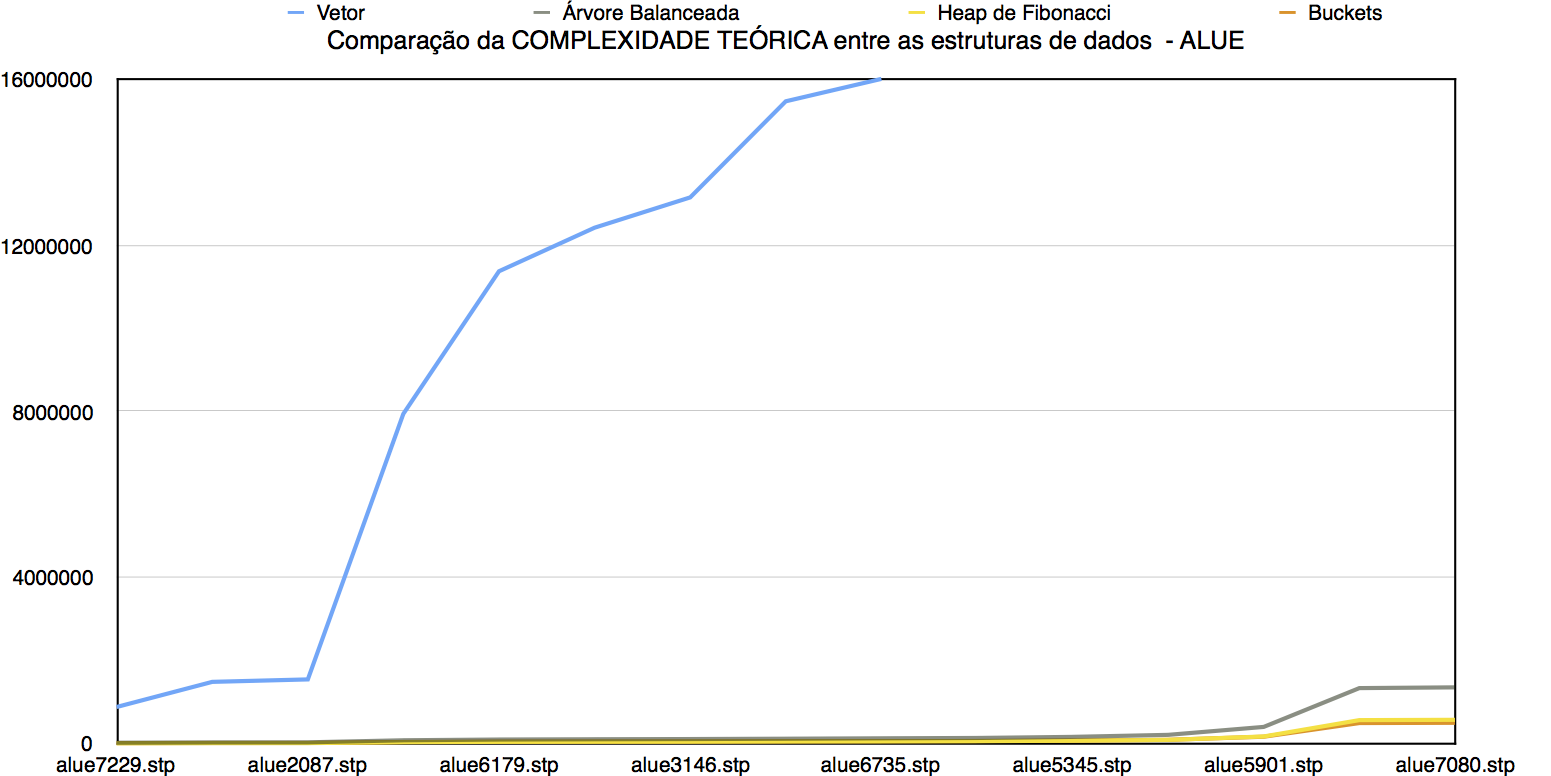
\includegraphics[width=6.4in]{charts/comp_teoria_alue.png}
 \caption{Gráfico comparativo das COMPLEXIDADES TEÓRICAS das estruturas de dados com as instâncias ALUE.}
 \label{fig:AlueGraphComplex}
\end{figure}

\begin{table}[H]
  \centering    
  \begin{tabular}{|c|r|r|r|r|r|r|r|}
    \toprule
    \multicolumn{4}{|c|}{\cellcolor{gray!25}\textbf{Árvore $\alpha$}} & \multicolumn{1}{|c|}{\cellcolor{gray!25}\textbf{$\alpha$ = 0.6}}     & \multicolumn{1}{|c|}{\cellcolor{gray!25}\textbf{$\alpha$ = 0.7}} & \multicolumn{1}{|c|}{\cellcolor{gray!25}\textbf{$\alpha$ = 0.8}} & \multicolumn{1}{|c|}{\cellcolor{gray!25}\textbf{$\alpha$ = 0.9}} \\
    \midrule
    \multicolumn{1}{|c|}{\cellcolor{gray!10}Arquivo} & \multicolumn{1}{|c|}{\cellcolor{gray!10}Vértices} & \multicolumn{1}{|c|}{\cellcolor{gray!10}Arestas} & \multicolumn{1}{|c|}{\cellcolor{gray!10}V. Processados} & 
    \multicolumn{1}{|c|}{\cellcolor{gray!10}Tempo} & \multicolumn{1}{|c|}{\cellcolor{gray!10}Tempo} &
    \multicolumn{1}{|c|}{\cellcolor{gray!10}Tempo} & \multicolumn{1}{|c|}{\cellcolor{gray!10}Tempo} \\
    % \midrule
    \hline
    alue7229	&	940	&	1474	&	809	&	0,001394	&	0,001439	&	0,001874	&	0,002653	\\
    \hline
    alue2105	&	1220	&	1858	&	896	&	0,001562	&	0,001633	&	0,002159	&	0,002995	\\
    \hline
    alue2087	&	1244	&	1971	&	933	&	0,001591	&	0,001657	&	0,002241	&	0,003251	\\
    \hline
    alue6951	&	2818	&	4419	&	2035	&	0,005416	&	0,005554	&	0,006596	&	0,008015	\\
    \hline
    alue6179	&	3372	&	5213	&	2748	&	0,006164	&	0,006590	&	0,008869	&	0,009958	\\
    \hline
    alue5067	&	3524	&	5560	&	2975	&	0,007102	&	0,007628	&	0,011092	&	0,011959	\\
    \hline
    alue3146	&	3626	&	5869	&	2852	&	0,006712	&	0,007080	&	0,010059	&	0,010731	\\
    \hline
    alue6457	&	3932	&	6137	&	3578	&	0,007822	&	0,008427	&	0,012173	&	0,014627	\\
    \hline
    alue6735	&	4119	&	6696	&	2970	&	0,007019	&	0,007576	&	0,010976	&	0,011811	\\
    \hline
    alue5623	&	4472	&	6938	&	2750	&	0,006452	&	0,006828	&	0,009103	&	0,010173	\\
    \hline
    alue5345	&	5179	&	8165	&	4215	&	0,008266	&	0,008907	&	0,012673	&	0,016955	\\
    \hline
    alue7066	&	6405	&	10454	&	4767	&	0,010225	&	0,010404	&	0,021761	&	0,023841	\\
    \hline
    alue5901	&	11543	&	18429	&	8579	&	0,016952	&	0,018853	&	0,115619	&	0,141570	\\
    \hline
    alue7065	&	34046	&	54841	&	31374	&	0,077132	&	0,083448	&	0,306071	&	0,357562	\\
    \hline
    alue7080	&	34479	&	55494	&	34479	&	0,085292	&	0,087687	&	0,486298	&	0,586772	\\
    \hline
  \end{tabular}
  \caption{Tabela de resultados do ALUE utilizando Árvore $\alpha$.}  
  \label{tab:AlueAlpha}
\end{table}

\begin{figure}[H]
 \centering
 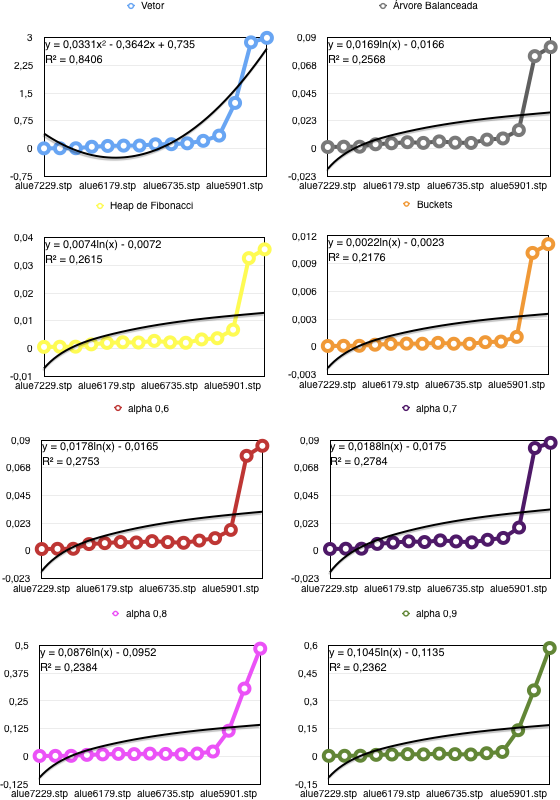
\includegraphics[width=6.4in]{charts/cpu_all_alue.png}
 \caption{TEMPO DE CPU das estruturas de dados executadas com as instâncias ALUE.}
 \label{fig:AlueGraphTime}
\end{figure}

\begin{figure}[H]
 \centering
 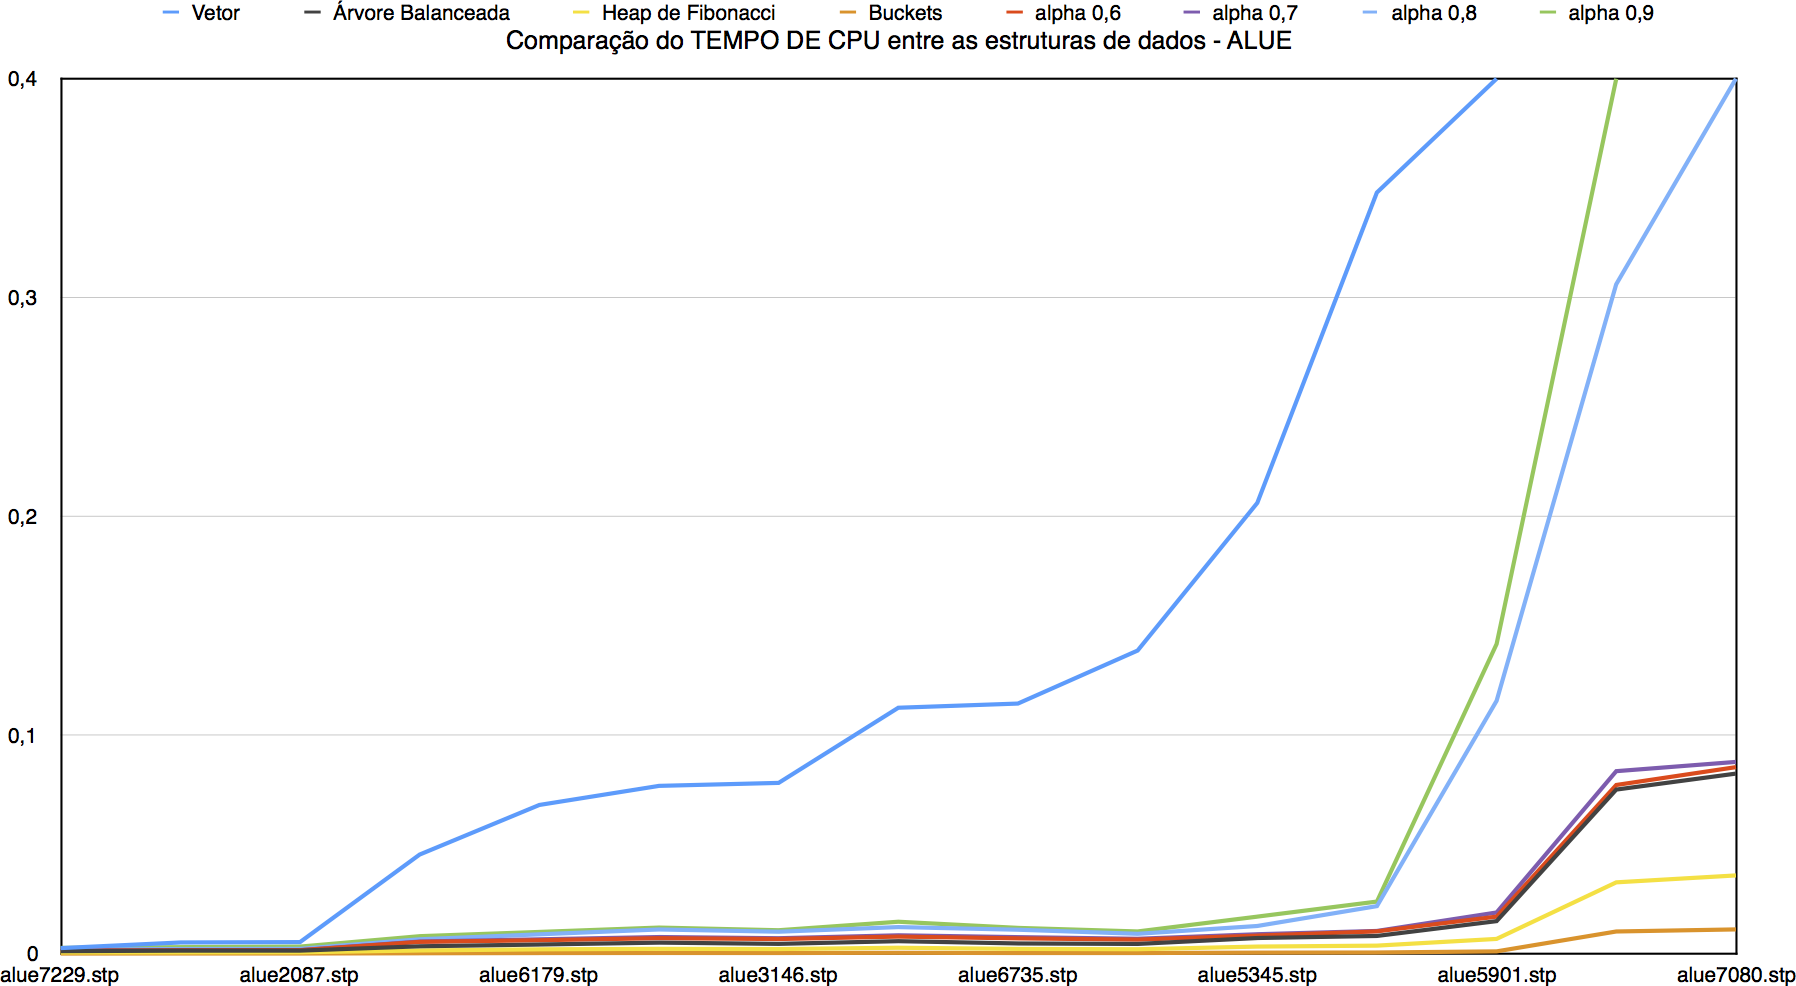
\includegraphics[width=6.4in]{charts/comp_ed_alue.png}
 \caption{Gráfico comparativo de TEMPO DE CPU das estruturas de dados executadas com as instâncias ALUE.}
 \label{fig:AlueGraphTimeAll}
\end{figure}

%%%%%%%%%%%%%%%%%%%%%%%%%%%%%%%%%%%%%%%%%%%%%%%%%%%%%%%%%%%%%%%%%%%%%%%%%%%%%

\begin{table}[H]
  \centering    
  \begin{tabular}{|c|r|r|r|r|r|}
    \toprule
    \multicolumn{5}{|c|}{\cellcolor{gray!25}\textbf{Vetor}} & \multicolumn{1}{|c|}{\cellcolor{gray!25}\textbf{Complexidade Teórica}}\\
    \midrule
    \multicolumn{1}{|c|}{\cellcolor{gray!10}Arquivo} & \multicolumn{1}{|c|}{\cellcolor{gray!10}Vértices} & \multicolumn{1}{|c|}{\cellcolor{gray!10}Arestas} & \multicolumn{1}{|c|}{\cellcolor{gray!10}V. Processados} & \multicolumn{1}{|c|}{\cellcolor{gray!10}Tempo} & \multicolumn{1}{|c|}{\cellcolor{gray!10}|V|\textsuperscript{2}}\\
    % \midrule
    \hline
    alut2764 & 387 & 626 & 387 & 0,000367 & 149769 \\
    \hline
    alut0805 & 966 & 1666 & 966 & 0,002558 & 933156 \\
    \hline
    alut0787 & 1160 & 2089 & 1160 & 0,003765 & 1345600 \\
    \hline
    alut1181 & 3041 & 5693 & 3041 & 0,050949 & 9247681 \\
    \hline
    alut2566 & 5021 & 9055 & 5021 & 0,178345 & 25210441 \\
    \hline
    alut2010 & 6104 & 11011 & 6104 & 0.306118 & 37258816 \\
    \hline
    alut2288 & 9070 & 16595 & 9070 & 0.696500 & 82264900 \\
    \hline
    alut2610 & 33901 & 62816 & 33901 & 2,794000 & 1149277801 \\
    \hline
    alut2625 & 36711 & 68117 & 36711 & 4,026000 & 1347697521 \\
    \hline
  \end{tabular}
  \caption{Tabela de resultados do ALUT utilizando Vetor.}  
  \label{tab:AlutVetor}
\end{table}

\begin{table}[H]
  \centering    
  \begin{tabular}{|c|r|r|r|r|r|}
    \toprule
    \multicolumn{5}{|c|}{\cellcolor{gray!25}\textbf{Árvore Balanceada de Busca}} & \multicolumn{1}{|c|}{\cellcolor{gray!25}\textbf{Complexidade Teórica}}\\
    \midrule
    \multicolumn{1}{|c|}{\cellcolor{gray!10}Arquivo} & \multicolumn{1}{|c|}{\cellcolor{gray!10}Vértices} & \multicolumn{1}{|c|}{\cellcolor{gray!10}Arestas} & \multicolumn{1}{|c|}{\cellcolor{gray!10}V. Processados} & \multicolumn{1}{|c|}{\cellcolor{gray!10}Tempo} & \multicolumn{1}{|c|}{\cellcolor{gray!10}(|V|+|E|)log|V|}\\
    % \midrule
    \hline
    alut2764	&	387	&	626	&	387	&	0,000552	&	8707,94	\\
    \hline
    alut0805	&	966	&	1666	&	956	&	0,001447	&	26098,59	\\
    \hline
    alut0787	&	1160	&	2089	&	1135	&	0,001702	&	33074,52	\\
    \hline
    alut1181	&	3041	&	5693	&	2465	&	0,003865	&	101055,26	\\
    \hline
    alut2566	&	5021	&	9055	&	3836	&	0,005875	&	173046,95	\\
    \hline
    alut2010	&	6104	&	11011	&	4729	&	0,007546	&	215230,35	\\
    \hline
    alut2288	&	9070	&	16595	&	8456	&	0,014194	&	337414,85	\\
    \hline
    alut2610	&	33901	&	62816	&	32746	&	0,070478	&	1455498,02	\\
    \hline
    alut2625	&	36711	&	68117	&	36702	&	0,079989	&	1589603,91	\\
    \hline
  \end{tabular}
  \caption{Tabela de resultados do ALUT utilizando Árvore Balanceada de Busca.}  
  \label{tab:AlutArvore}
\end{table}


\begin{table}[H]
  \centering    
  \begin{tabular}{|c|r|r|r|r|r|}
    \toprule
    \multicolumn{5}{|c|}{\cellcolor{gray!25}\textbf{Heap de Fibonacci}} & \multicolumn{1}{|c|}{\cellcolor{gray!25}\textbf{Complexidade Teórica}}\\
    \midrule
    \multicolumn{1}{|c|}{\cellcolor{gray!10}Arquivo} & \multicolumn{1}{|c|}{\cellcolor{gray!10}Vértices} & \multicolumn{1}{|c|}{\cellcolor{gray!10}Arestas} & \multicolumn{1}{|c|}{\cellcolor{gray!10}V. Processados} & \multicolumn{1}{|c|}{\cellcolor{gray!10}Tempo} & \multicolumn{1}{|c|}{\cellcolor{gray!10}|V|log|V| + E}\\
    % \midrule
    \hline
    alut2764 &	387	&	626	&	387	&	0,000240	&	3952,73	\\
    \hline
    alut0805 &	966	&	1666	&	956	&	0,000658	&	11244,74	\\
    \hline
    alut0787 &	1160	&	2089	&	1135	&	0,000774	&	13897,69	\\
    \hline
    alut1181 &	3041	&	5693	&	2465	&	0,001757	&	40878,37	\\
    \hline
    alut2566 &	5021	&	9055	&	3836	&	0,002798	&	70781,96	\\
    \hline
    alut2010 &	6104	&	11011	&	4729	&	0,003430	&	87772,09	\\
    \hline
    alut2288 &	9070	&	16595	&	8456	&	0,006452	&	135837,26	\\
    \hline
    alut2610 &	33901	&	62816	&	32746	&	0,030643	&	572993,51	\\
    \hline
    alut2625 &	36711	&	68117	&	36702	&	0,034778	&	624799,84	\\
    \hline
  \end{tabular}
  \caption{Tabela de resultados do ALUT utilizando Heap de Fibonacci.}  
  \label{tab:AlutHeap}
\end{table}


\begin{table}[H]
  \centering    
  \begin{tabular}{|c|r|r|r|r|r|r|}
    \toprule
    \multicolumn{6}{|c|}{\cellcolor{gray!25}\textbf{Buckets}} & \multicolumn{1}{|c|}{\cellcolor{gray!25}\textbf{Complexidade Teórica}}\\
    \midrule
    \multicolumn{1}{|c|}{\cellcolor{gray!10}Arquivo} & \multicolumn{1}{|c|}{\cellcolor{gray!10}Vértices} & \multicolumn{1}{|c|}{\cellcolor{gray!10}Arestas} & \multicolumn{1}{|c|}{\cellcolor{gray!10}V. Processados} & \multicolumn{1}{|c|}{\cellcolor{gray!10}C} &
    \multicolumn{1}{|c|}{\cellcolor{gray!10}Tempo} & \multicolumn{1}{|c|}{\cellcolor{gray!10}|V|C + |E|}\\
    % \midrule
    \hline
    alut2764 & 387 & 626 & 387 & 13 & 0,000035 & 5657,00 \\
    \hline
    alut0805 & 966 & 1666 & 956 & 13 & 0,000078 & 14224,00 \\
    \hline
    alut0787 & 1160 & 2089 & 1135 & 13 & 0,000102 & 17169,00 \\
    \hline
    alut1181 & 3041 & 5693 & 2465 & 13 & 0,000219 & 45226,00 \\
    \hline
    alut2566 & 5021 & 9055 & 3836 & 13 & 0,000373 & 74328,00 \\
    \hline
    alut2010 & 6104 & 11011 & 4729 & 13 & 0,000461 & 90363,00 \\
    \hline
    alut2288 & 9070 & 16595 & 8456 & 13 & 0,000875 & 134505,00 \\
    \hline
    alut2610 & 33901 & 62816 & 32746 & 13 & 0,007657 & 503529,00 \\
    \hline
    alut2625 & 36711 & 68117 & 36702 & 13 & 0,009155 & 545360,00 \\
    \hline
  \end{tabular}
  \caption{Tabela de resultados do ALUT utilizando Buckets.}  
  \label{tab:AlutBuckets}
\end{table}

\begin{figure}[!ht]
 \centering
 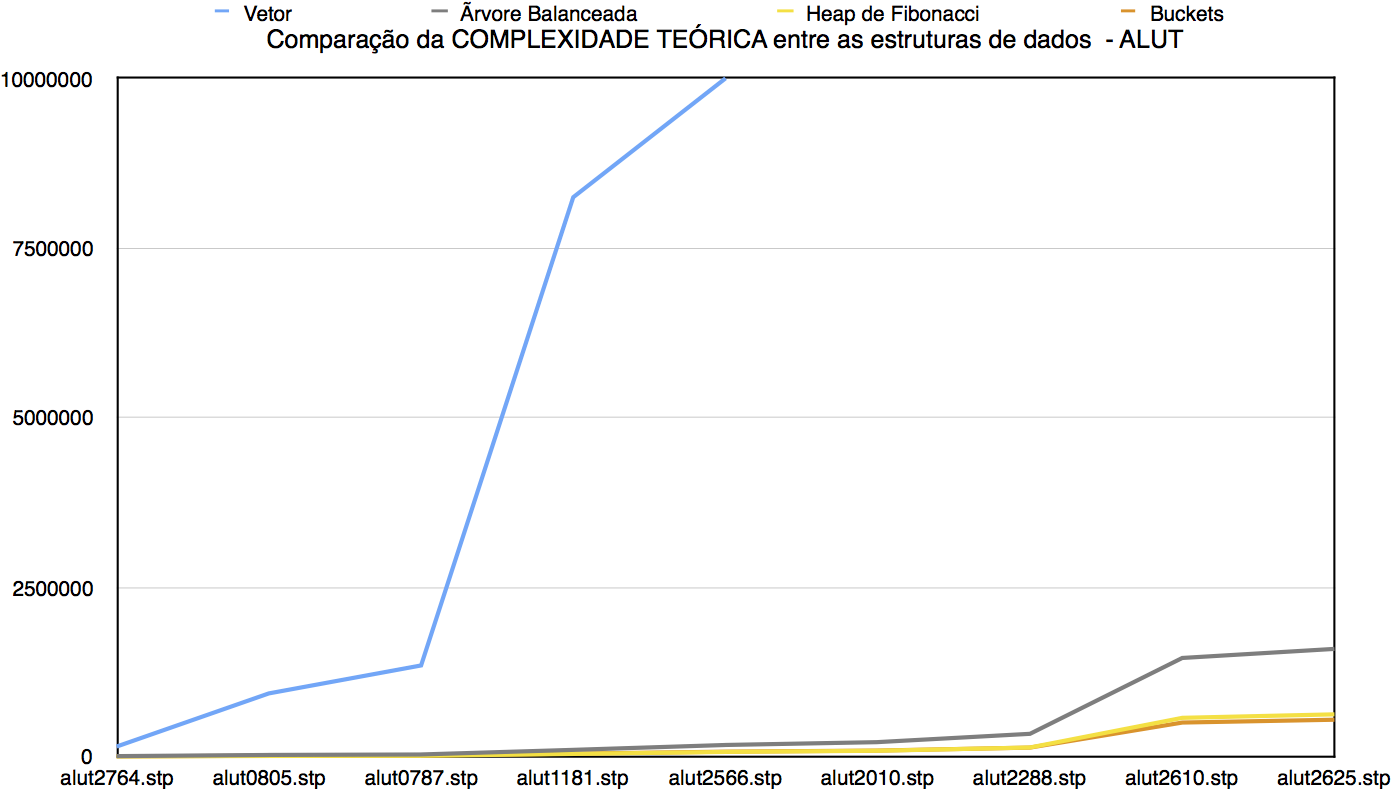
\includegraphics[width=6.4in]{charts/comp_teoria_alut.png}
 \caption{Gráfico comparativo das COMPLEXIDADES TEÓRICAS das estruturas de dados com as instâncias ALUT.}
 \label{fig:AlutGraphComplex}
\end{figure}

\begin{table}[H]
  \centering    
  \begin{tabular}{|c|r|r|r|r|r|r|r|}
    \toprule
    \multicolumn{4}{|c|}{\cellcolor{gray!25}\textbf{Árvore $\alpha$}} & \multicolumn{1}{|c|}{\cellcolor{gray!25}\textbf{$\alpha$ = 0.6}}     & \multicolumn{1}{|c|}{\cellcolor{gray!25}\textbf{$\alpha$ = 0.7}} & \multicolumn{1}{|c|}{\cellcolor{gray!25}\textbf{$\alpha$ = 0.8}} & \multicolumn{1}{|c|}{\cellcolor{gray!25}\textbf{$\alpha$ = 0.9}} \\
    \midrule
    \multicolumn{1}{|c|}{\cellcolor{gray!10}Arquivo} & \multicolumn{1}{|c|}{\cellcolor{gray!10}Vértices} & \multicolumn{1}{|c|}{\cellcolor{gray!10}Arestas} & \multicolumn{1}{|c|}{\cellcolor{gray!10}V. Processados} & 
    \multicolumn{1}{|c|}{\cellcolor{gray!10}Tempo} & \multicolumn{1}{|c|}{\cellcolor{gray!10}Tempo} &
    \multicolumn{1}{|c|}{\cellcolor{gray!10}Tempo} & \multicolumn{1}{|c|}{\cellcolor{gray!10}Tempo} \\
    % \midrule
    \hline
    alut2764	&	387	&	626	&	387	&	0,000875	&	0,000908	&	0,001107	&	0,001187	\\
    \hline
    alut0805	&	966	&	1666	&	956	&	0,001812	&	0,001893	&	0,002965	&	0,003833	\\
    \hline
    alut0787	&	1160	&	2089	&	1135	&	0,002563	&	0,002663	&	0,002849	&	0,003428	\\
    \hline
    alut1181	&	3041	&	5693	&	2465	&	0,005778	&	0,005999	&	0,008133	&	0,012162	\\
    \hline
    alut2566	&	5021	&	9055	&	3836	&	0,007988	&	0,008059	&	0,015542	&	0,016673	\\
    \hline
    alut2010	&	6104	&	11011	&	4729	&	0,008669	&	0,008797	&	0,018705	&	0,026794	\\
    \hline
    alut2288	&	9070	&	16595	&	8456	&	0,016335	&	0,016554	&	0,028892	&	0,035797	\\
    \hline
    alut2610	&	33901	&	62816	&	32746	&	0,072391	&	0,074272	&	0,162042	&	0,235736	\\
    \hline
    alut2625	&	36711	&	68117	&	36702	&	0,081993	&	0,083734	&	0,180950	&	0,303431	\\
    \hline
  \end{tabular}
  \caption{Tabela de resultados do ALUT utilizando Árvore $\alpha$ (com $\alpha$ = 0.6).}  
  \label{tab:AlutAlpha0.6}
\end{table}

\begin{figure}[H]
 \centering
 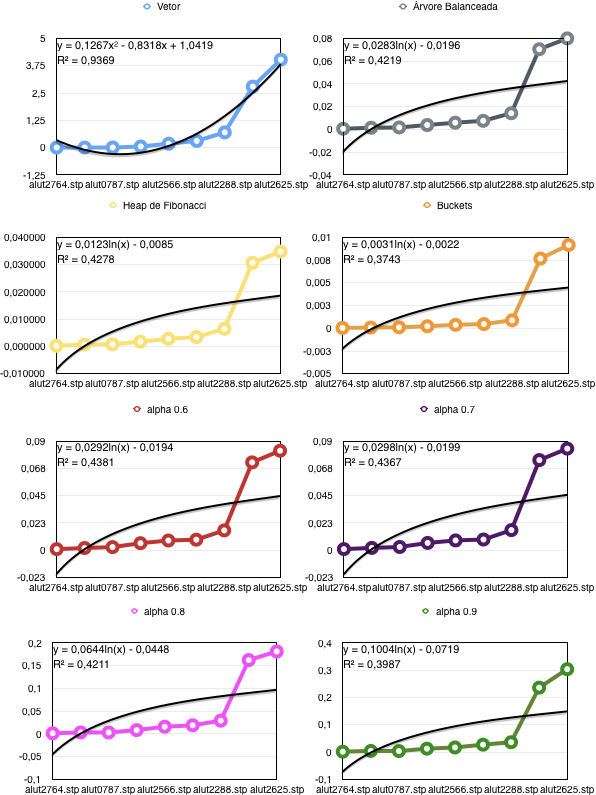
\includegraphics[width=6.4in]{charts/cpu_all_alut.png}
 \caption{TEMPO DE CPU das estruturas de dados executadas com as instâncias ALUT.}
 \label{fig:AlutGraphTime}
\end{figure}

\begin{figure}[H]
 \centering
 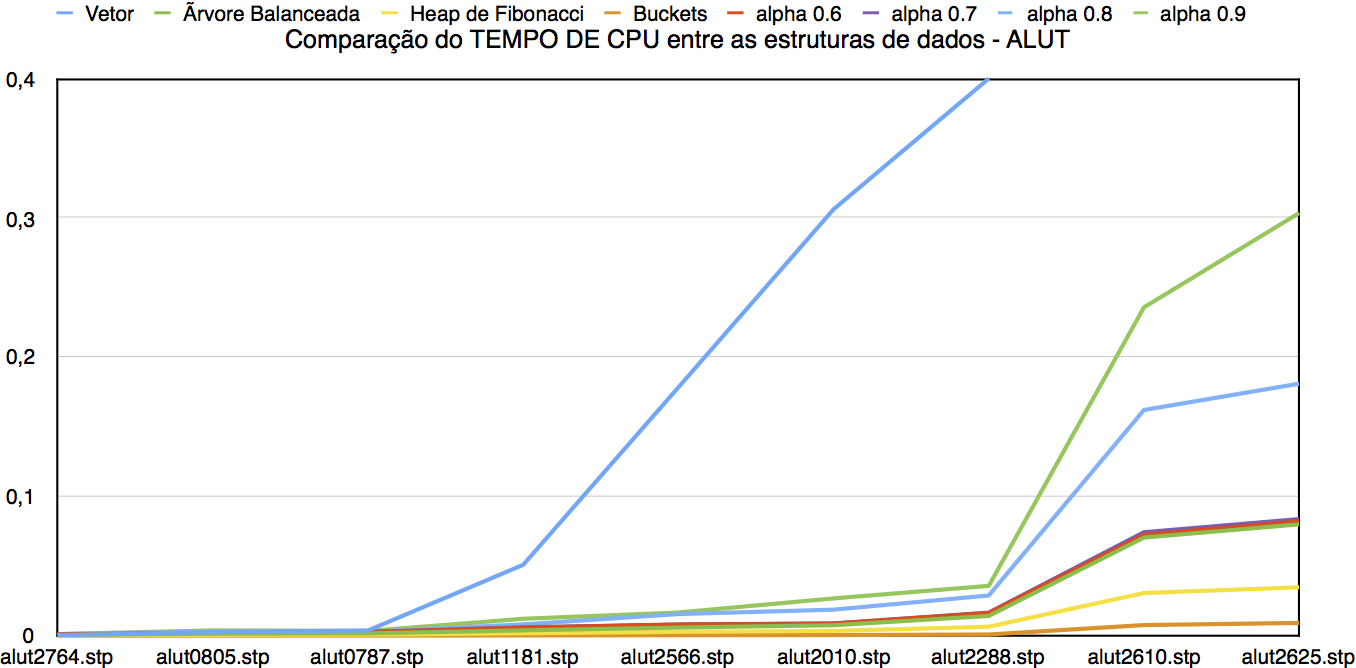
\includegraphics[width=6.4in]{charts/comp_ed_alut.png}
 \caption{Gráfico comparativo de TEMPO DE CPU das estruturas de dados executadas com as instâncias ALUT.}
 \label{fig:AlutGraphTimeAll}
\end{figure}


%%%%%%%%%%%%%%%%%%%%%%%%%%%%%%%%%%%%%%%%%%%%%%%%%%%%%%%%%%%%%%%%%%%%%%%%%%%%%

\begin{table}[H]
  \centering    
  \begin{tabular}{|c|r|r|r|r|r|}
    \toprule
    \multicolumn{5}{|c|}{\cellcolor{gray!25}\textbf{Vetor}} & \multicolumn{1}{|c|}{\cellcolor{gray!25}\textbf{Complexidade Teórica}}\\
    \midrule
    \multicolumn{1}{|c|}{\cellcolor{gray!10}Arquivo} & \multicolumn{1}{|c|}{\cellcolor{gray!10}Vértices} & \multicolumn{1}{|c|}{\cellcolor{gray!10}Arestas} & \multicolumn{1}{|c|}{\cellcolor{gray!10}V. Processados} & \multicolumn{1}{|c|}{\cellcolor{gray!10}Tempo} & \multicolumn{1}{|c|}{\cellcolor{gray!10}|V|\textsuperscript{2}}\\
    % \midrule
    \hline
    dmxa0628	&	169	&	280	&	169	&	0,000091	&	28561	\\
    \hline
    dmxa0296	&	233	&	386	&	233	&	0,000147	&	54289	\\
    \hline
    dmxa1304	&	298	&	503	&	298	&	0,000268	&	88804	\\
    \hline
    dmxa1109	&	343	&	559	&	343	&	0,000316	&	117649	\\
    \hline
    dmxa0848	&	499	&	861	&	499	&	0,000749	&	249001	\\
    \hline
    dmxa0903	&	632	&	1087	&	632	&	0,001125	&	399424	\\
    \hline
    dmxa0734	&	663	&	1154	&	663	&	0,001228	&	439569	\\
    \hline
    dmxa1516	&	720	&	1269	&	720	&	0,001468	&	518400	\\
    \hline
    dmxa1200	&	770	&	1383	&	770	&	0,001749	&	592900	\\
    \hline
    dmxa1721	&	1005	&	1731	&	1005	&	0,002817	&	1010025	\\
    \hline
    dmxa0454	&	1848	&	3286	&	1848	&	0,017255	&	3415104	\\
    \hline
    dmxa0368	&	2050	&	3676	&	2050	&	0,022631	&	4202500	\\
    \hline
    dmxa1801	&	2333	&	4137	&	2333	&	0,031400	&	5442889	\\
    \hline
    dmxa1010	&	3983	&	7108	&	3983	&	0,101520	&	15864289	\\    
    \hline
  \end{tabular}
  \caption{Tabela de resultados do DMXA utilizando Vetor.}  
  \label{tab:DmxaVetor}
\end{table}

\begin{table}[H]
  \centering    
  \begin{tabular}{|c|r|r|r|r|r|}
    \toprule
    \multicolumn{5}{|c|}{\cellcolor{gray!25}\textbf{Árvore Balanceada de Busca}} & \multicolumn{1}{|c|}{\cellcolor{gray!25}\textbf{Complexidade Teórica}}\\
    \midrule
    \multicolumn{1}{|c|}{\cellcolor{gray!10}Arquivo} & \multicolumn{1}{|c|}{\cellcolor{gray!10}Vértices} & \multicolumn{1}{|c|}{\cellcolor{gray!10}Arestas} & \multicolumn{1}{|c|}{\cellcolor{gray!10}V. Processados} & \multicolumn{1}{|c|}{\cellcolor{gray!10}Tempo} & \multicolumn{1}{|c|}{\cellcolor{gray!10}(|V|+|E|)log|V|}\\
    % \midrule
    \hline
    dmxa0628	&	169	&	280	&	169	&	0,000218	&	3322,99	\\
    \hline
    dmxa0296	&	233	&	386	&	178	&	0,000228	&	4867,93	\\
    \hline
    dmxa1304	&	298	&	503	&	298	&	0,000415	&	6583,55	\\
    \hline
    dmxa1109	&	343	&	559	&	343	&	0,000506	&	7596,70	\\
    \hline
    dmxa0848	&	499	&	861	&	455	&	0,000690	&	12189,54	\\
    \hline
    dmxa0903	&	632	&	1087	&	588	&	0,000875	&	15993,20	\\
    \hline
    dmxa0734	&	663	&	1154	&	663	&	0,000969	&	17030,50	\\
    \hline
    dmxa1516	&	720	&	1269	&	646	&	0,001009	&	18879,30	\\
    \hline
    dmxa1200	&	770	&	1383	&	713	&	0,001012	&	20644,50	\\
    \hline
    dmxa1721	&	1005	&	1731	&	751	&	0,001207	&	27286,07	\\
    \hline
    dmxa0454	&	1848	&	3286	&	911	&	0,001272	&	55712,88	\\
    \hline
    dmxa0368	&	2050	&	3676	&	2033	&	0,003019	&	62994,06	\\
    \hline
    dmxa1801	&	2333	&	4137	&	1821	&	0,002816	&	72386,17	\\
    \hline
    dmxa1010	&	3983	&	7108	&	3778	&	0,005940	&	132644,36	\\
    \hline
  \end{tabular}
  \caption{Tabela de resultados do DMXA utilizando Árvore Balanceada de Busca.}  
  \label{tab:DmxaArvore}
\end{table}


\begin{table}[H]
  \centering    
  \begin{tabular}{|c|r|r|r|r|r|}
    \toprule
    \multicolumn{5}{|c|}{\cellcolor{gray!25}\textbf{Heap de Fibonacci}} & \multicolumn{1}{|c|}{\cellcolor{gray!25}\textbf{Complexidade Teórica}}\\
    \midrule
    \multicolumn{1}{|c|}{\cellcolor{gray!10}Arquivo} & \multicolumn{1}{|c|}{\cellcolor{gray!10}Vértices} & \multicolumn{1}{|c|}{\cellcolor{gray!10}Arestas} & \multicolumn{1}{|c|}{\cellcolor{gray!10}V. Processados} & \multicolumn{1}{|c|}{\cellcolor{gray!10}Tempo} & \multicolumn{1}{|c|}{\cellcolor{gray!10}|V|log|V| + E}\\
    % \midrule
    \hline
    dmxa0628	&	169	&	280	&	169	&	0,000104	&	1530,75	\\
    \hline
    dmxa0296	&	233	&	386	&	178	&	0,000109	&	2218,36	\\
    \hline
    dmxa1304	&	298	&	503	&	298	&	0,000189	&	2952,31	\\
    \hline
    dmxa1109	&	343	&	559	&	343	&	0,000221	&	3447,77	\\
    \hline
    dmxa0848	&	499	&	861	&	455	&	0,000300	&	5333,49	\\
    \hline
    dmxa0903	&	632	&	1087	&	588	&	0,000398	&	6966,99	\\
    \hline
    dmxa0734	&	663	&	1154	&	663	&	0,000451	&	7368,21	\\
    \hline
    dmxa1516	&	720	&	1269	&	646	&	0,000439	&	8103,13	\\
    \hline
    dmxa1200	&	770	&	1383	&	713	&	0,000482	&	8766,31	\\
    \hline
    dmxa1721	&	1005	&	1731	&	751	&	0,000503	&	11753,84	\\
    \hline
    dmxa0454	&	1848	&	3286	&	911	&	0,000606	&	23340,03	\\
    \hline
    dmxa0368	&	2050	&	3676	&	2033	&	0,001438	&	26228,89	\\
    \hline
    dmxa1801	&	2333	&	4137	&	1821	&	0,001280	&	30238,54	\\
    \hline
    dmxa1010	&	3983	&	7108	&	3778	&	0,002829	&	54743,25	\\
    \hline
  \end{tabular}
  \caption{Tabela de resultados do DMXA utilizando Heap de Fibonacci.}  
  \label{tab:DmxaHeap}
\end{table}


\begin{table}[H]
  \centering    
  \begin{tabular}{|c|r|r|r|r|r|r|}
    \toprule
    \multicolumn{6}{|c|}{\cellcolor{gray!25}\textbf{Buckets}} & \multicolumn{1}{|c|}{\cellcolor{gray!25}\textbf{Complexidade Teórica}}\\
    \midrule
    \multicolumn{1}{|c|}{\cellcolor{gray!10}Arquivo} & \multicolumn{1}{|c|}{\cellcolor{gray!10}Vértices} & \multicolumn{1}{|c|}{\cellcolor{gray!10}Arestas} & \multicolumn{1}{|c|}{\cellcolor{gray!10}V. Processados} & \multicolumn{1}{|c|}{\cellcolor{gray!10}C} &
    \multicolumn{1}{|c|}{\cellcolor{gray!10}Tempo} & \multicolumn{1}{|c|}{\cellcolor{gray!10}|V|C + |E|}\\
    % \midrule
    \hline
    dmxa0628	&	169	&	280	&	169	&	13	&	0,000015	&	2477	\\
    \hline
    dmxa0296	&	233	&	386	&	178	&	13	&	0,000019	&	3415	\\
    \hline
    dmxa1304	&	298	&	503	&	298	&	13	&	0,000025	&	4377	\\
    \hline
    dmxa1109	&	343	&	559	&	343	&	13	&	0,000029	&	5018	\\
    \hline
    dmxa0848	&	499	&	861	&	455	&	13	&	0,000037	&	7348	\\
    \hline
    dmxa0903	&	632	&	1087	&	588	&	13	&	0,000050	&	9303	\\
    \hline
    dmxa0734	&	663	&	1154	&	663	&	13	&	0,000056	&	9773	\\
    \hline
    dmxa1516	&	720	&	1269	&	646	&	13	&	0,000058	&	10629	\\
    \hline
    dmxa1200	&	770	&	1383	&	713	&	13	&	0,000062	&	11393	\\
    \hline
    dmxa1721	&	1005	&	1731	&	751	&	13	&	0,000070	&	14796	\\
    \hline
    dmxa0454	&	1848	&	3286	&	911	&	13	&	0,000086	&	27310	\\
    \hline
    dmxa0368	&	2050	&	3676	&	2033	&	13	&	0,000194 &	30326	\\
    \hline
    dmxa1801	&	2333	&	4137	&	1821	&	13	&	0,000169 &	34466	\\
    \hline
    dmxa1010	&	3983	&	7108	&	3778	&	13	&	0,000363 &	58887	\\   
    \hline
  \end{tabular}
  \caption{Tabela de resultados do DMXA utilizando Buckets.}  
  \label{tab:DmxaBuckets}
\end{table}

\begin{figure}[H]
 \centering
 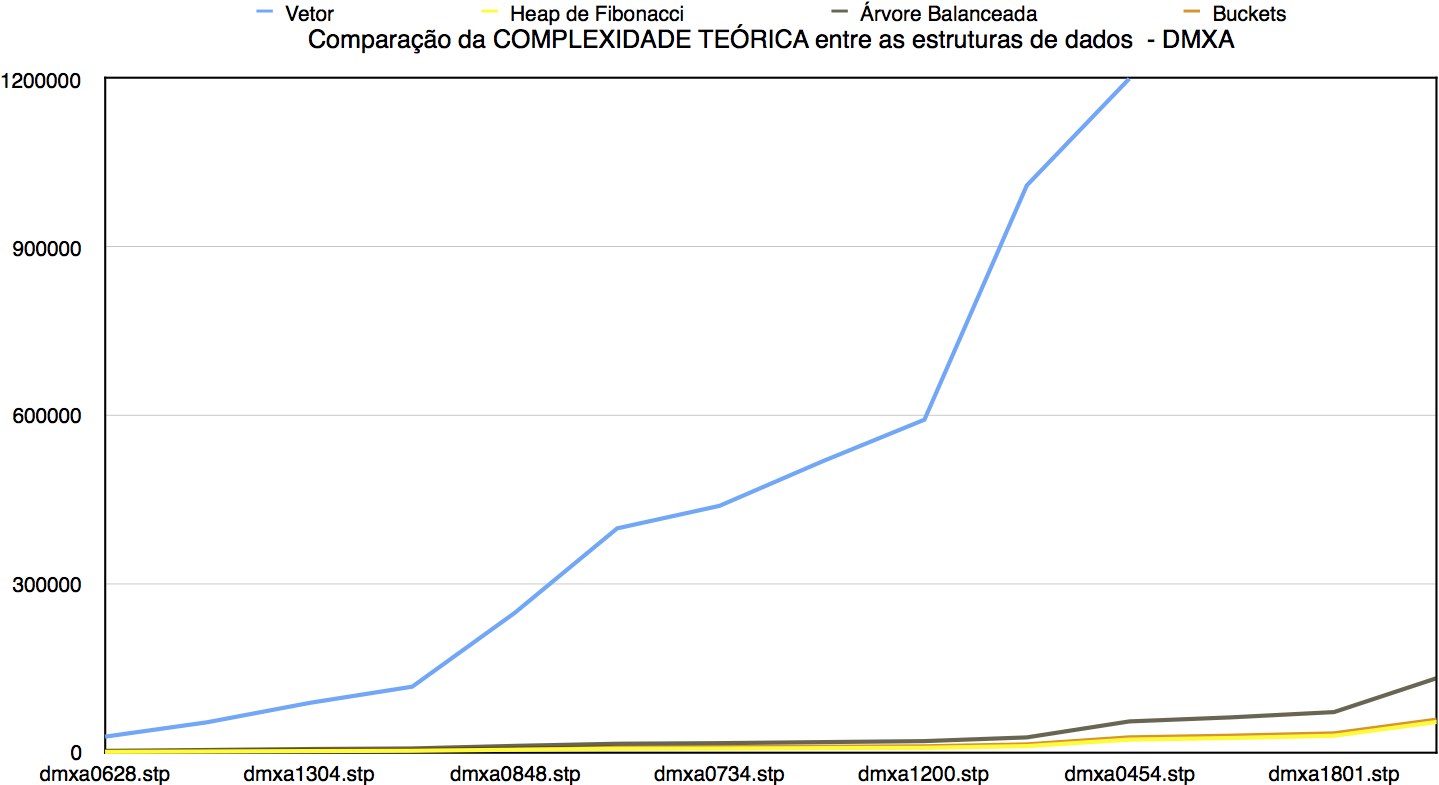
\includegraphics[width=6.4in]{charts/comp_teoria_dmxa.png}
 \caption{Gráfico comparativo das COMPLEXIDADES TEÓRICAS das estruturas de dados com as instâncias DMXA.}
 \label{fig:DmxaGraphComplex}
\end{figure}

\begin{table}[ht!]
  \centering    
  \begin{tabular}{|c|r|r|r|r|r|r|r|}
    \toprule
    \multicolumn{4}{|c|}{\cellcolor{gray!25}\textbf{Árvore $\alpha$}} & \multicolumn{1}{|c|}{\cellcolor{gray!25}\textbf{$\alpha$ = 0.6}}     & \multicolumn{1}{|c|}{\cellcolor{gray!25}\textbf{$\alpha$ = 0.7}} & \multicolumn{1}{|c|}{\cellcolor{gray!25}\textbf{$\alpha$ = 0.8}} & \multicolumn{1}{|c|}{\cellcolor{gray!25}\textbf{$\alpha$ = 0.9}} \\
    \midrule
    \multicolumn{1}{|c|}{\cellcolor{gray!10}Arquivo} & \multicolumn{1}{|c|}{\cellcolor{gray!10}Vértices} & \multicolumn{1}{|c|}{\cellcolor{gray!10}Arestas} & \multicolumn{1}{|c|}{\cellcolor{gray!10}V. Processados} & 
    \multicolumn{1}{|c|}{\cellcolor{gray!10}Tempo} & \multicolumn{1}{|c|}{\cellcolor{gray!10}Tempo} &
    \multicolumn{1}{|c|}{\cellcolor{gray!10}Tempo} & \multicolumn{1}{|c|}{\cellcolor{gray!10}Tempo} \\
    % \midrule
    \hline    
    dmxa0628	&	169	&	280	&	169	&	0,000723	&	0,000745	&	0,0008050	&	0,0008360	\\
    \hline
    dmxa0296	&	233	&	386	&	178	&	0,000732	&	0,000754	&	0,0008090	&	0,0008550	\\
    \hline
    dmxa1304	&	298	&	503	&	298	&	0,000927	&	0,000949	&	0,0011330	&	0,0011850	\\
    \hline
    dmxa1109	&	343	&	559	&	343	&	0,001002	&	0,001029	&	0,0011970	&	0,0012760	\\
    \hline
    dmxa0848	&	499	&	861	&	455	&	0,001215	&	0,001228	&	0,0014660	&	0,0016830	\\
    \hline
    dmxa0903	&	632	&	1087	&	588	&	0,001382	&	0,001399	&	0,0017030	&	0,0019540	\\
    \hline
    dmxa0734	&	663	&	1154	&	663	&	0,001447	&	0,001471	&	0,0018280	&	0,0021920	\\
    \hline
    dmxa1516	&	720	&	1269	&	646	&	0,001409	&	0,001441	&	0,0017980	&	0,0021570	\\
    \hline
    dmxa1200	&	770	&	1383	&	713	&	0,001512	&	0,001607	&	0,0018890	&	0,0023150	\\
    \hline
    dmxa1721	&	1005	&	1731	&	751	&	0,001707	&	0,001857	&	0,0021000	&	0,0026040	\\
    \hline
    dmxa0454	&	1848	&	3286	&	911	&	0,001985	&	0,002481	&	0,0040000	&	0,0051770	\\
    \hline
    dmxa0368	&	2050	&	3676	&	2033	&	0,004529	&	0,004922	&	0,0065850	&	0,0079870	\\
    \hline
    dmxa1801	&	2333	&	4137	&	1821	&	0,004023	&	0,004287	&	0,0058130	&	0,0073610	\\
    \hline
    dmxa1010	&	3983	&	7108	&	3778	&	0,008125	&	0,008469	&	0,0112490	&	0,0152190	\\
    \hline
  \end{tabular}
  \caption{Tabela de resultados do DMXA utilizando Árvore $\alpha$ (com $\alpha$ = 0.6).}  
  \label{tab:DmxaAlpha0.6}
\end{table}

\begin{figure}
 \centering
 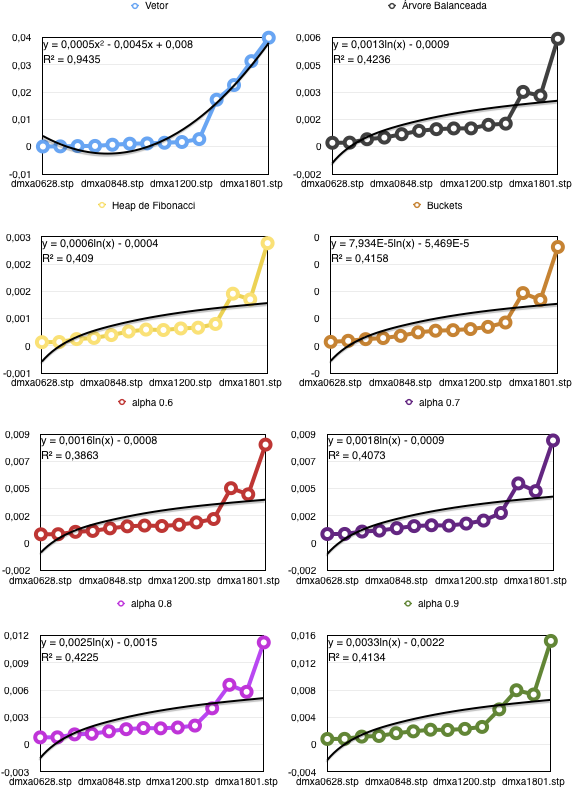
\includegraphics[width=6.4in]{charts/cpu_all_dmxa.png}
 \caption{TEMPO DE CPU das estruturas de dados executadas com as instâncias DMXA.}
 \label{fig:DmxaGraphTime}
\end{figure}

\begin{figure}[H]
 \centering
 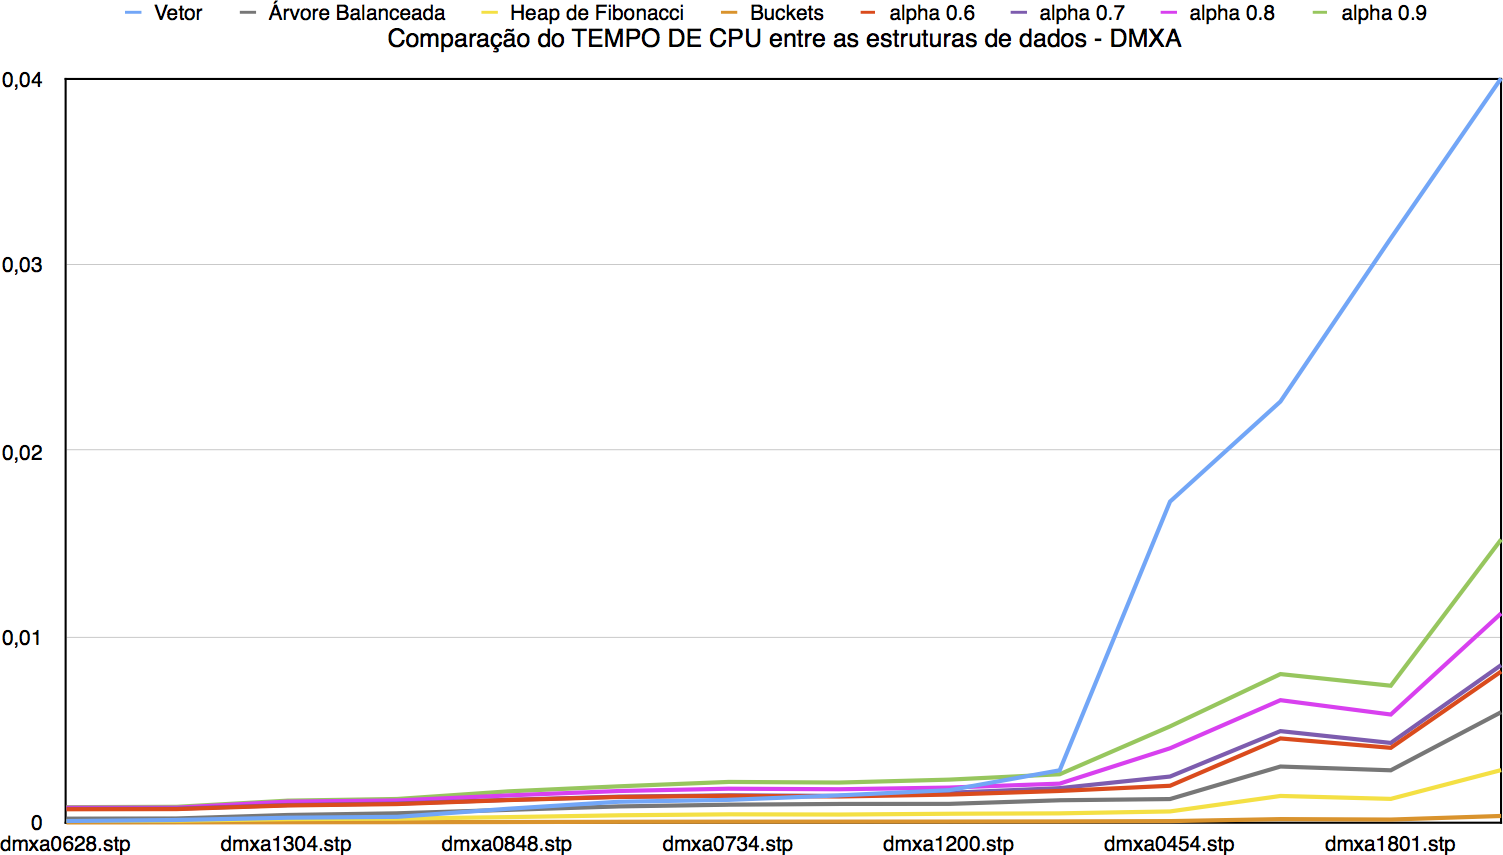
\includegraphics[width=6.4in]{charts/comp_ed_dmxa.png}
 \caption{Gráfico comparativo de TEMPO DE CPU das estruturas de dados executadas com as instâncias DMXA.}
 \label{fig:AlueGraphTimeAll}
\end{figure}

As figuras \ref{fig:AlueGraphTime},  \ref{fig:AlutGraphTime}, \ref{fig:DmxaGraphTime},    mostram como se comportou o algoritmo com diferentes estruturas de dados. Em preto, desenhamos uma linha de tendência de acordo com a complexidade teórica calculada. Em algoritmos polinomiais, desenhamos uma função polinomial, e nos demais desenhamos uma função envolvendo logaritmos em função do número de vértices.

Nota-se uma elevação no tempo das última instâncias em relação a linha de tendência logarítmica apresentada. Isso deve-se ao fato de que a última instância apresenta um crescimento desproporcional no número de arestas, o que não é contabilizado pelas funções tendência apresentadas. Isso ocorre pois os gráficos foram ilustrados em 2 dimensões, o que impossibilita múltiplas variáveis.

% ---
% Finaliza a parte no bookmark do PDF, para que se inicie o bookmark na raiz
% ---
\bookmarksetup{startatroot}% 
% ---

% ---
% Conclusão
% ---
\chapter*[Conclusão]{Conclusão}
\addcontentsline{toc}{chapter}{Conclusão}


Para todas as instâncias, obteve-se a complexidade teórica e desempenho esperado para cada operação utilizada com as estruturas de dados, como mostram as tabelas da Seção de Resultados. Ao comparar o tempo de CPU, é possivel notar a seguinte hierarquia: \textbf{Buckets < Heap de Fibonacci < Árvore Balanceada de Busca < Árvore $\alpha$(0.6) <  Árvore $\alpha$(0.7) <  Árvore $\alpha$(0.8) <  Árvore $\alpha$(0.9) < Vetor}.

Em grafos densos, o número de arestas é proporcional a $n^2$. Essa hierarquia nos resultados, e as complexidades analisadas nos capítulos anteriores (tabela abaixo), mostram que o input usado neste trabalho era composto de grafos não tão densos.

\begin{table}[ht!]
\centering    
    \begin{tabular}{|c|c|c|c|c|c|c|}
    \hline
    \multicolumn{1}{|c|}{\cellcolor{gray!10} Operações} & \multicolumn{1}{|c|}{\cellcolor{gray!10}Vetor} & \multicolumn{1}{|c|}{\cellcolor{gray!10}Árvore BB} & \multicolumn{1}{|c|}{\cellcolor{gray!10}H. de Fibonacci} & \multicolumn{1}{|c|}{\cellcolor{gray!10}Buckets}\\ %& \multicolumn{1}{|c|}{\cellcolor{gray!10}Árvore $\alpha$}\\
    \hline
    Inicializar & O($n$) & O($n.log(n)$) & O($n$) & O($n$) %& O($n.(log(n) +\alpha n)\le n^2$)
    \\
    \hline
    RemoverMin & O($n^2$) & O($n.log(n)$) & O($n.log(n)$) & O($nC$) %& O($n.(1+log(\alpha n)$)
    \\
    \hline
    Atualizar & O($n^2$) & O($m.log(n)$) & O($m$) & O($m$) %& O($m.(1+log(\alpha n))$)
    \\
    \hline
    Total & O($n^2$) & O($(n+m).log(n)$) & O($n.log(n)+m$) & O($nC + m$) %& O($(n+m).(1+log(\alpha n)$)
    \\    
    \hline
    \end{tabular}
    \caption{Tabela com o resumo das complexidades teórica.}  
    \label{tab:complex}
\end{table}

Observa-se que a inicialização do algoritmo tem menor complexidade que o seu corpo. Assim, essa inicialização não influencia a complexidade final. A complexidade depende predominantemente do custo de se remover o menor elemento e de se atualizar um elemento na estrutura, e do tamanho/densidade do grafo.

Os resultados mostraram que os desempenhos do algoritmo Dijkstra com o uso de Heap de Fibonacci e Buckets são próximos para quantidades pequenas de vértices. O desempenho do Buckets supera o Heap de Fibonacci para quantidades grandes de vértices, isso deve-se ao limite superior de $nC$ iterações definidos pelo algoritmo, já que para todos os arquivos de entrada, a aresta com maior peso era sempre C=13.

É importante notar que, com o uso de Buckets, o algoritmo é pseudo-polinomial em relação a aresta com maior peso. Portanto, com C constante temos uma complexidade O($n+m$), que supera a complexidade de O($n.logn + m$) do Heap de Fibonacci. Caso não soubéssemos de antemão o comprimento máximo da representação do tamanho de uma aresta, seria inviável fixar a constante C, e o Buckets não teria performance melhor que as outras estruturas de dados.

Em seguida, nota-se que o desempenho da Árvore Balanceada de Busca é bem superior ao Vetor. Caso os grafos de entrada fossem densos, o número de arestas seria proporcional a $n^2$, o que faria a Árvore Balanceada de Busca custar O($n^2.log(n)$), superior a complexidade total do Vetor. Mais uma vez, podemos notar que os grafos de entrada não eram muito densos.

% Acho que temos que colocar algum gráfico comparando todas as estruturas aqui, pra facilitar a visualização dessa conclusão sobre os resultados

Conforme analisado na seção 1.5, a complexidade do algoritmo Dijkstra com o uso da árvore-$\alpha$ varia entre O($(n+m).log(n)$) e O($n^2$) para 1/2 $<$ $\alpha$ $<l$ 1. Isso foi corroborado pelos resultados obtidos na execução do algoritmo para os valores 0.6, 0.7, 0.8 e 0.9. É visível o crescimento do tempo de CPU conforme o aumento do $\alpha$, onde: $\alpha$=0.6 é limite superior de O($(n+m).log(n)$) da Árvore Balanceada de Busca; E $\alpha$=0.9, é limitado superiormente pelo O($n^2$) do Vetor.

%retirei a árvore alfa porque não tenho menor ideia de como fazer a formula dela... Só sei que se aproxima de vetor n^2 para alpha proximo de 1 e da árvore heap para alfa proximo a 0,5. Deixei a tabela a seguir, mas se não fecharmos essa fórmula, acho melhor remover. 


%\begin{table}[ht!]
%\centering    
%    \begin{tabular}{|c|c|c|c|c|c|}
%    \hline
%    \multicolumn{1}{|c|}{\cellcolor{gray!10} Operações} &  %\multicolumn{1}{|c|}{\cellcolor{gray!10}Árvore $\alpha$}\\
%    \hline
%    Inicializar & O($n.(log(n) +\alpha n)\le n^2$)\\
%    \hline
%    RemoverMin &  O($n.(1+log(\alpha n)$)\\
%    \hline
%    Atualizar &  O($m.(1+log(\alpha n))$)\\
%    \hline
%    Total & O($(n+m).(1+log(\alpha n)$)\\    
%    \hline
%    \end{tabular}
%    \caption{Tabela com o resumo das complexidades teórica.}  
%    \label{tab:complex_alfa}
%\end{table}




% ----------------------------------------------------------
% Referências bibliográficas
% ----------------------------------------------------------
\bibliography{abntex2-modelo-references}


% ----------------------------------------------------------
% Apêndices
% ----------------------------------------------------------
% Inicia os apêndices
% ---
% \begin{apendicesenv}

% \chapter{Lorem Ipsum}

% \end{apendicesenv}


% ----------------------------------------------------------
% Anexos
% ----------------------------------------------------------
% % Inicia os anexos
% ---
% \begin{anexosenv}

% \chapter{Lorem Ipsum}

% \end{anexosenv}


\printindex

\end{document}


% Este documento e seu código-fonte são exemplos de referência de uso da classe
% \textsf{abntex2} e do pacote \textsf{abntex2cite}. O documento 
% exemplifica a elaboração de relatórios técnicos e/ou científicos produzidos
% conforme a ABNT NBR 10719:2011 \emph{Informação e documentação - Relatório
% técnico e/ou científico - Apresentação}.

% A expressão ``Modelo canônico'' é utilizada para indicar que \abnTeX\ não é
% modelo específico de nenhuma universidade ou instituição, mas que implementa tão
% somente os requisitos das normas da ABNT. Uma lista completa das normas
% observadas pelo \abnTeX\ é apresentada em \citeonline{abntex2classe}.

% Sinta-se convidado a participar do projeto \abnTeX! Acesse o site do projeto em
% \url{http://abntex2.googlecode.com/}. Também fique livre para conhecer,
% estudar, alterar e redistribuir o trabalho do \abnTeX, desde que os arquivos
% modificados tenham seus nomes alterados e que os créditos sejam dados aos
% autores originais, nos termos da ``The \LaTeX\ Project Public
% License''\footnote{\url{http://www.latex-project.org/lppl.txt}}.

% Encorajamos que sejam realizadas customizações específicas deste exemplo para
% universidades e outras instituições --- como capas, folhas de rosto, etc.
% Porém, recomendamos que ao invés de se alterar diretamente os arquivos do
% \abnTeX, distribua-se arquivos com as respectivas customizações.
% Isso permite que futuras versões do \abnTeX~não se tornem automaticamente
% incompatíveis com as customizações promovidas. Consulte
% \citeonline{abntex2-wiki-como-customizar} par mais informações.

% Este documento deve ser utilizado como complemento dos manuais do \abnTeX\ 
% \cite{abntex2classe,abntex2cite,abntex2cite-alf} e da classe \textsf{memoir}
% \cite{memoir}. 